\chapter{Anexo}
\label{cap:anexo}

\begin{figure}[ht!]
  \section{Álvaro Gómez Sittima}
  \label{sec:disenyoAlvaro}
  \begin{subfigure}{\textwidth}
    \centering
    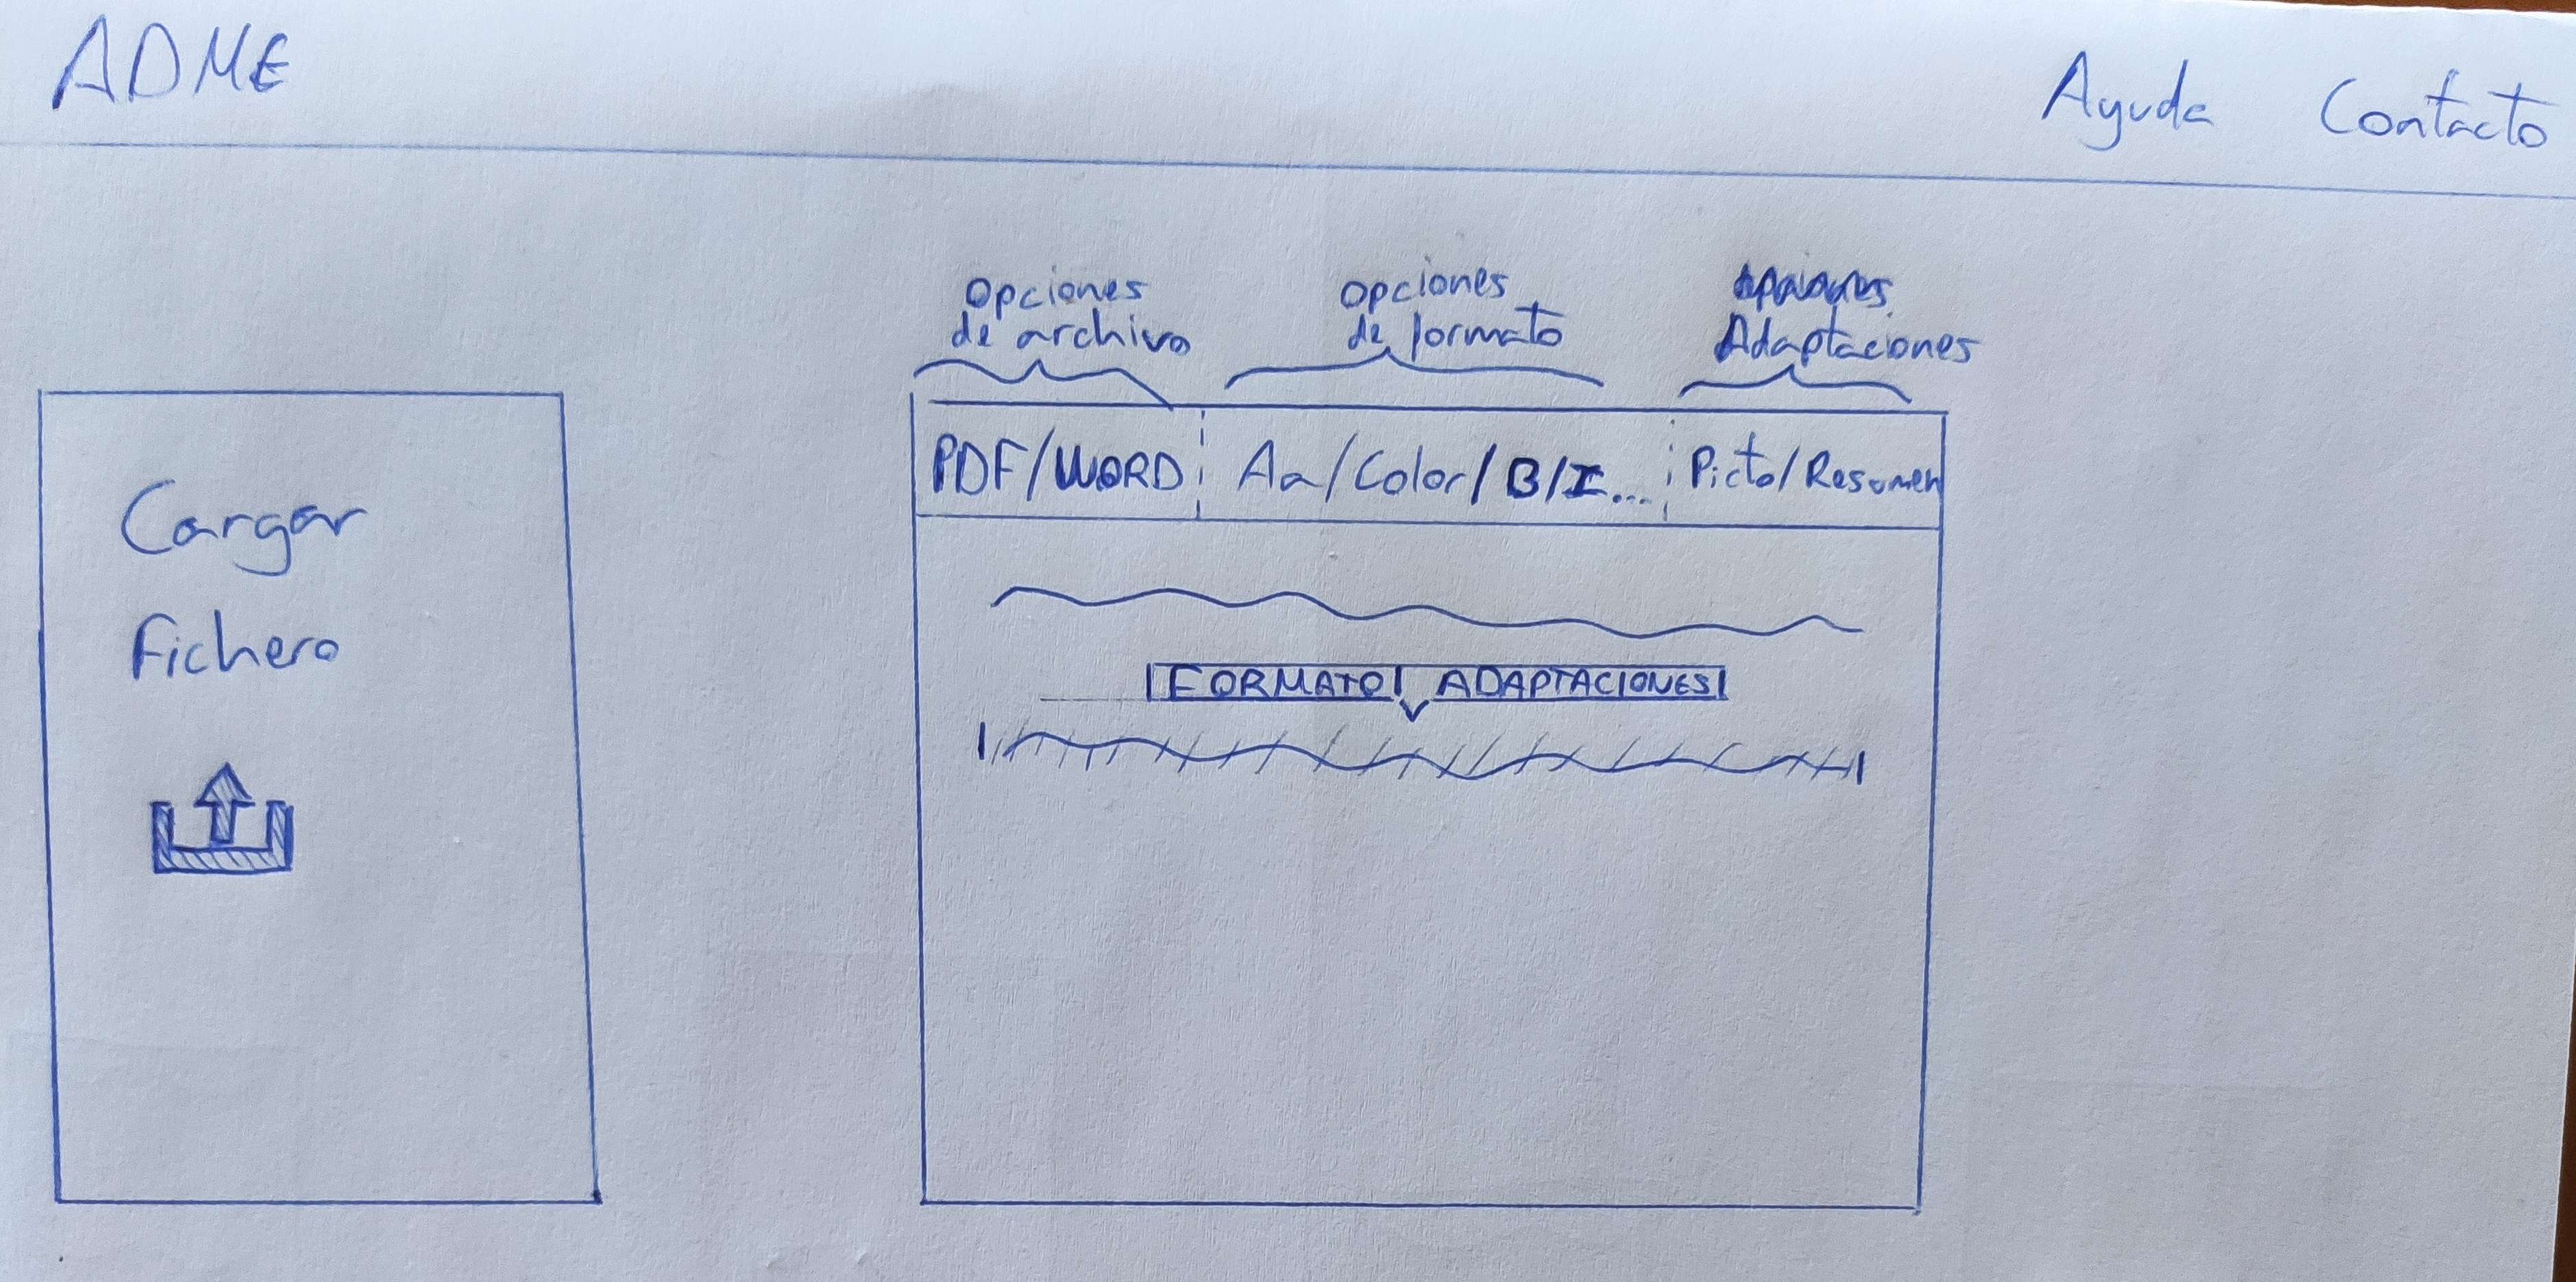
\includegraphics[width=0.7\textwidth]{Diseño/Alvaro/Alvaro01.jpg}
    \caption{Diseño pantalla de inicio de Álvaro sin PDF.}
    \label{fig:disenyoAlvaro01}
  \end{subfigure}

  \begin{subfigure}{\textwidth}
    \centering
    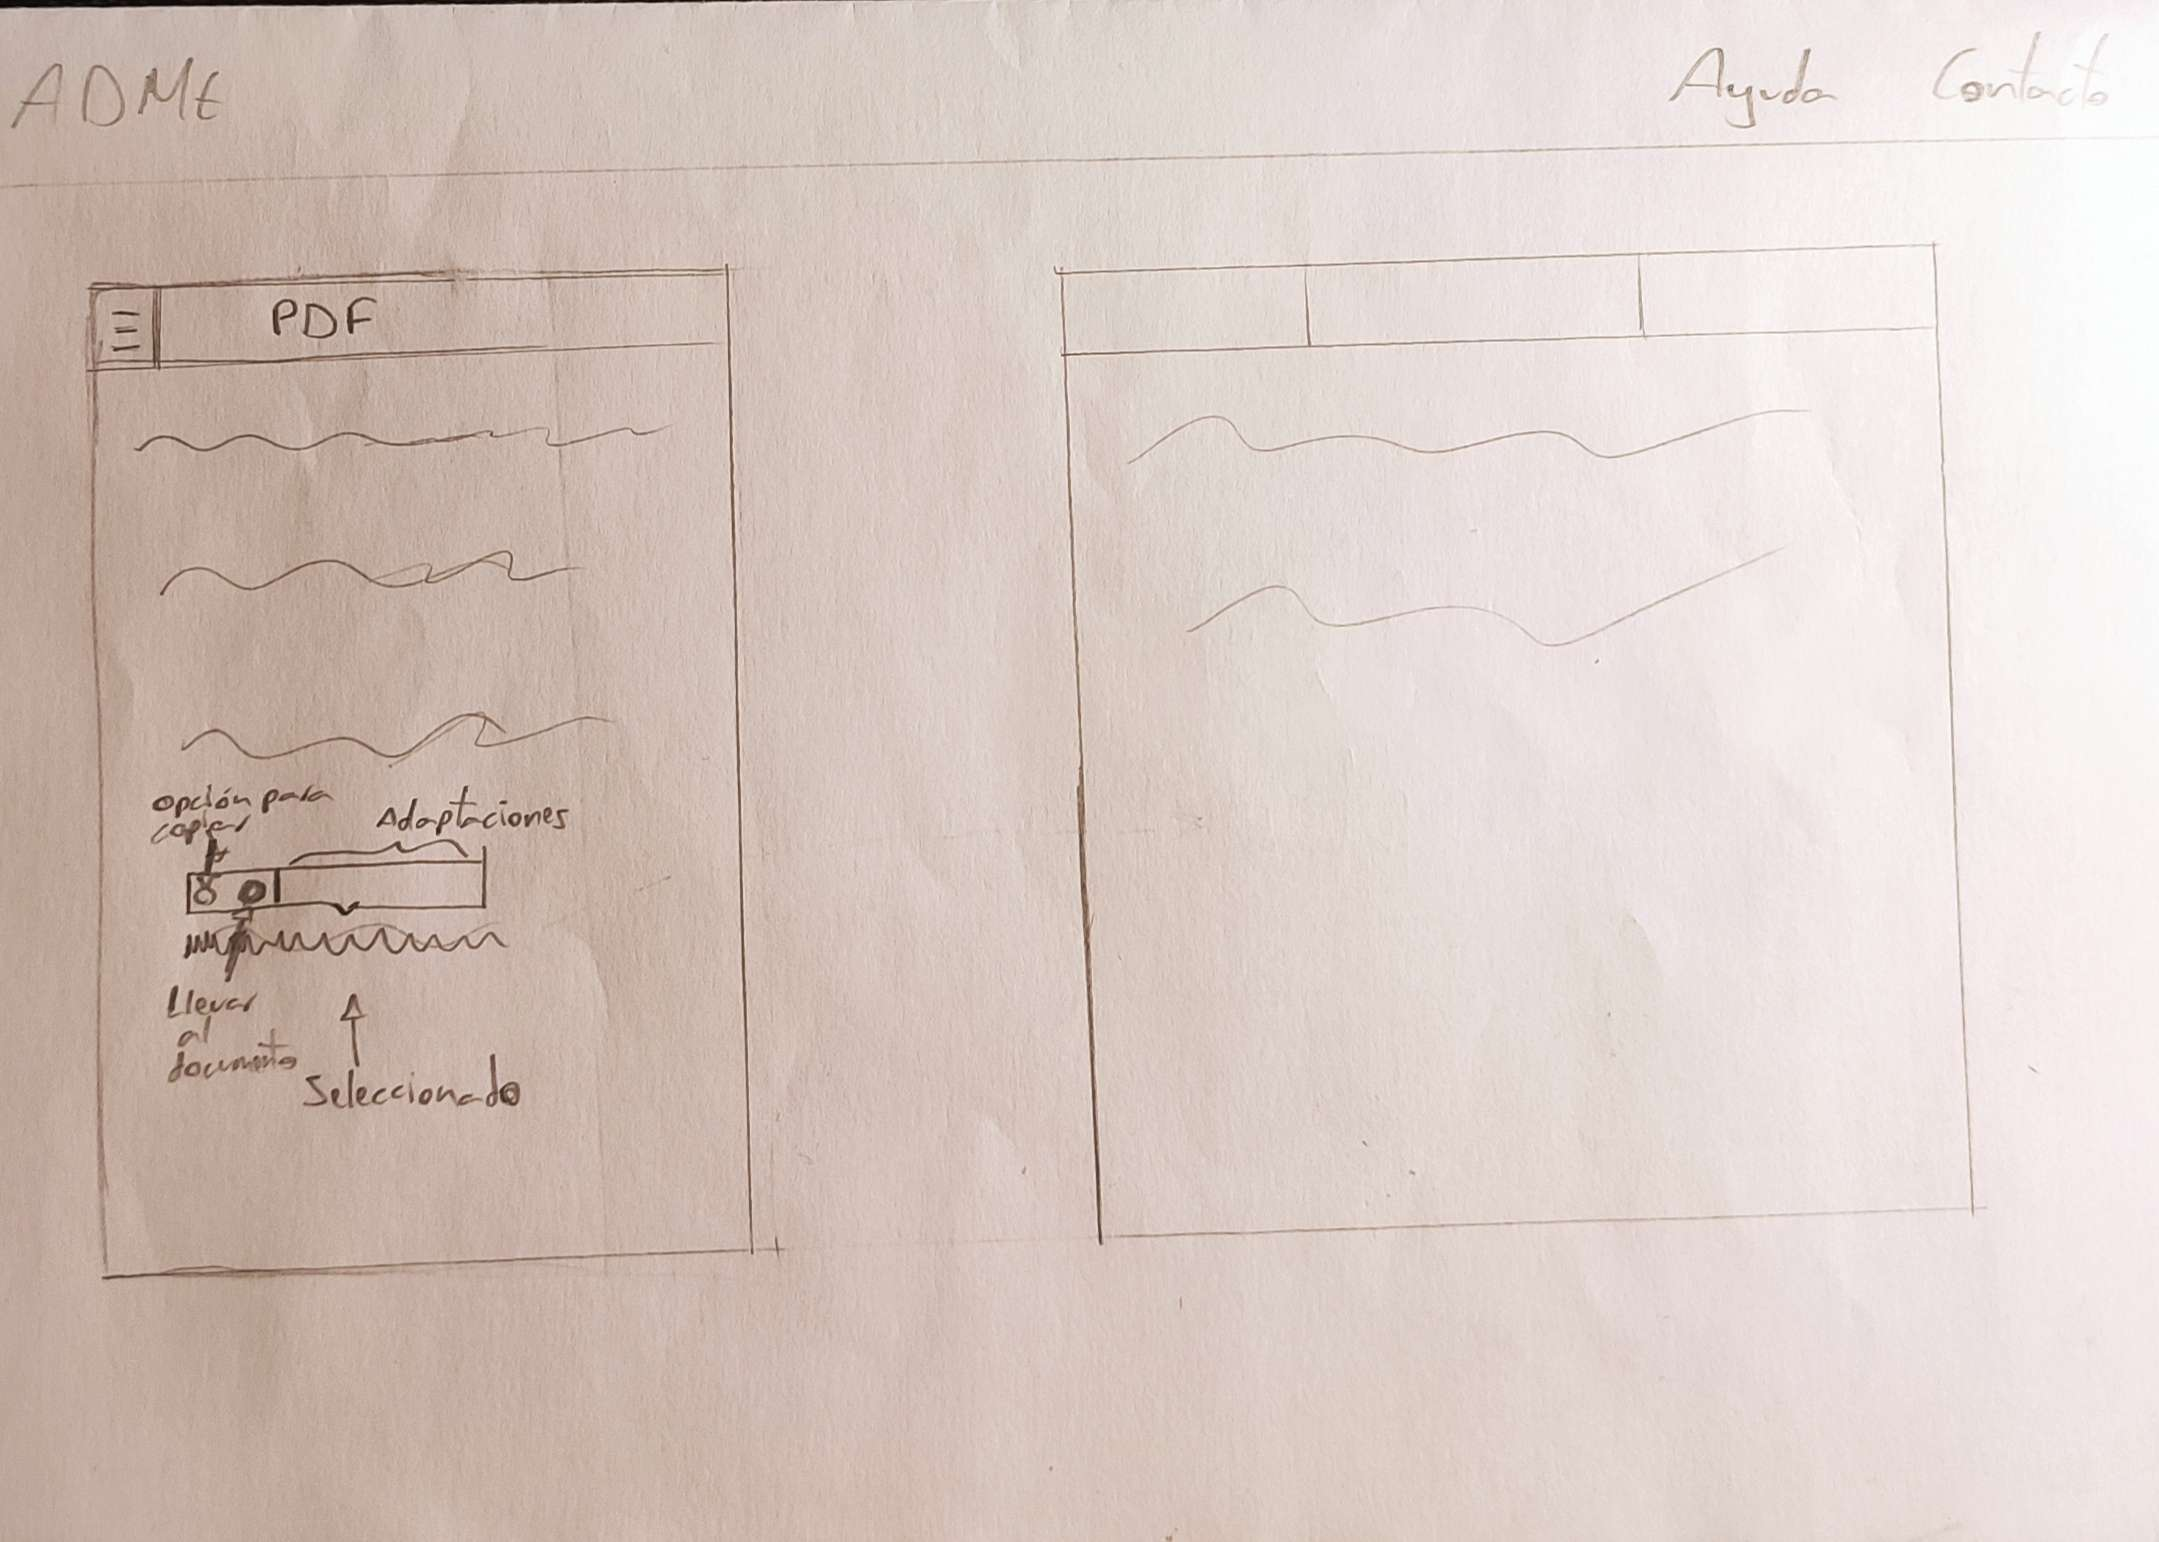
\includegraphics[width=0.7\textwidth]{Diseño/Alvaro/Alvaro02.jpg}
    \caption{Diseño pantalla de inicio de Álvaro con PDF.}
    \label{fig:disenyoAlvaro02}
  \end{subfigure}
  \caption{Diseños de Álvaro Gómez Sittima}
  \label{fig:disenyoAlvaro}
\end{figure}

\begin{figure}[ht!]
  \ContinuedFloat

  \begin{subfigure}{\textwidth}
    \centering
    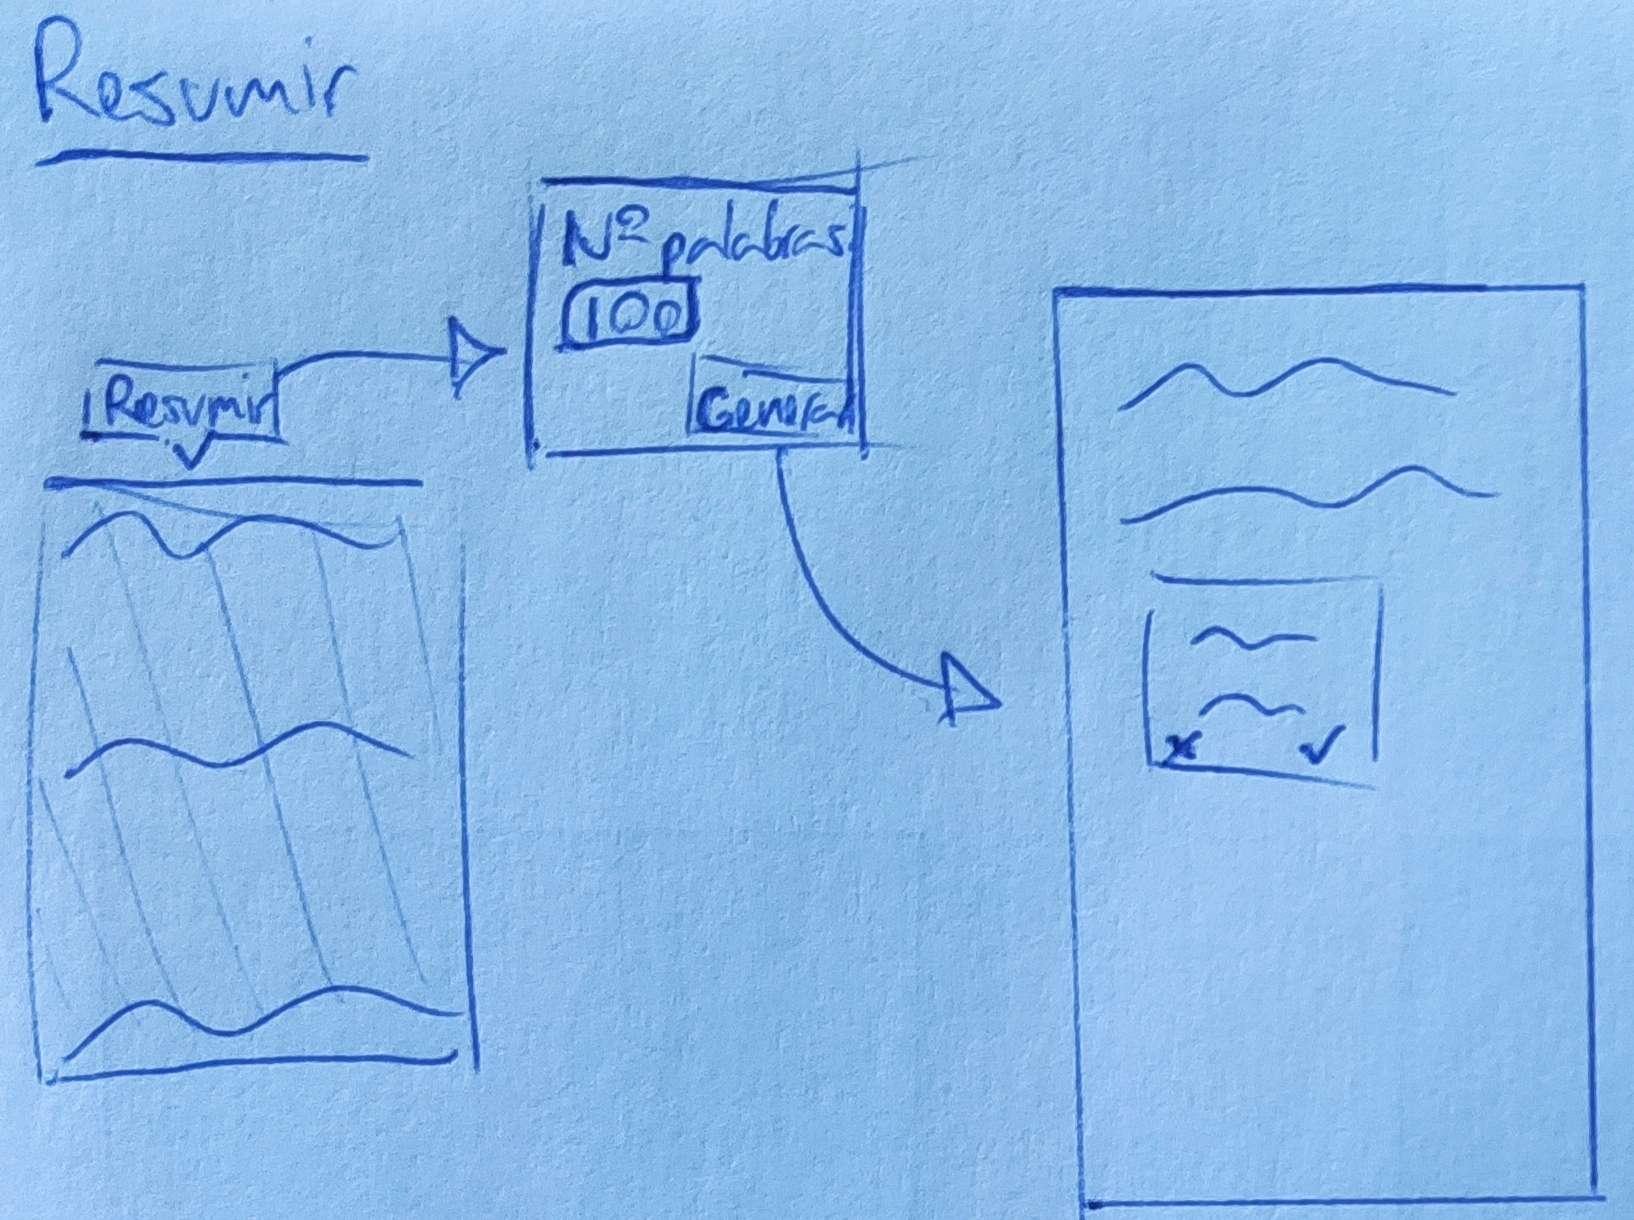
\includegraphics[width=0.6\textwidth]{Diseño/Alvaro/Alvaro03.jpg}
    \caption{Diseño generar resumen de Álvaro.}
    \label{fig:disenyoAlvaro03}
  \end{subfigure}

  \begin{subfigure}{\textwidth}
    \centering
    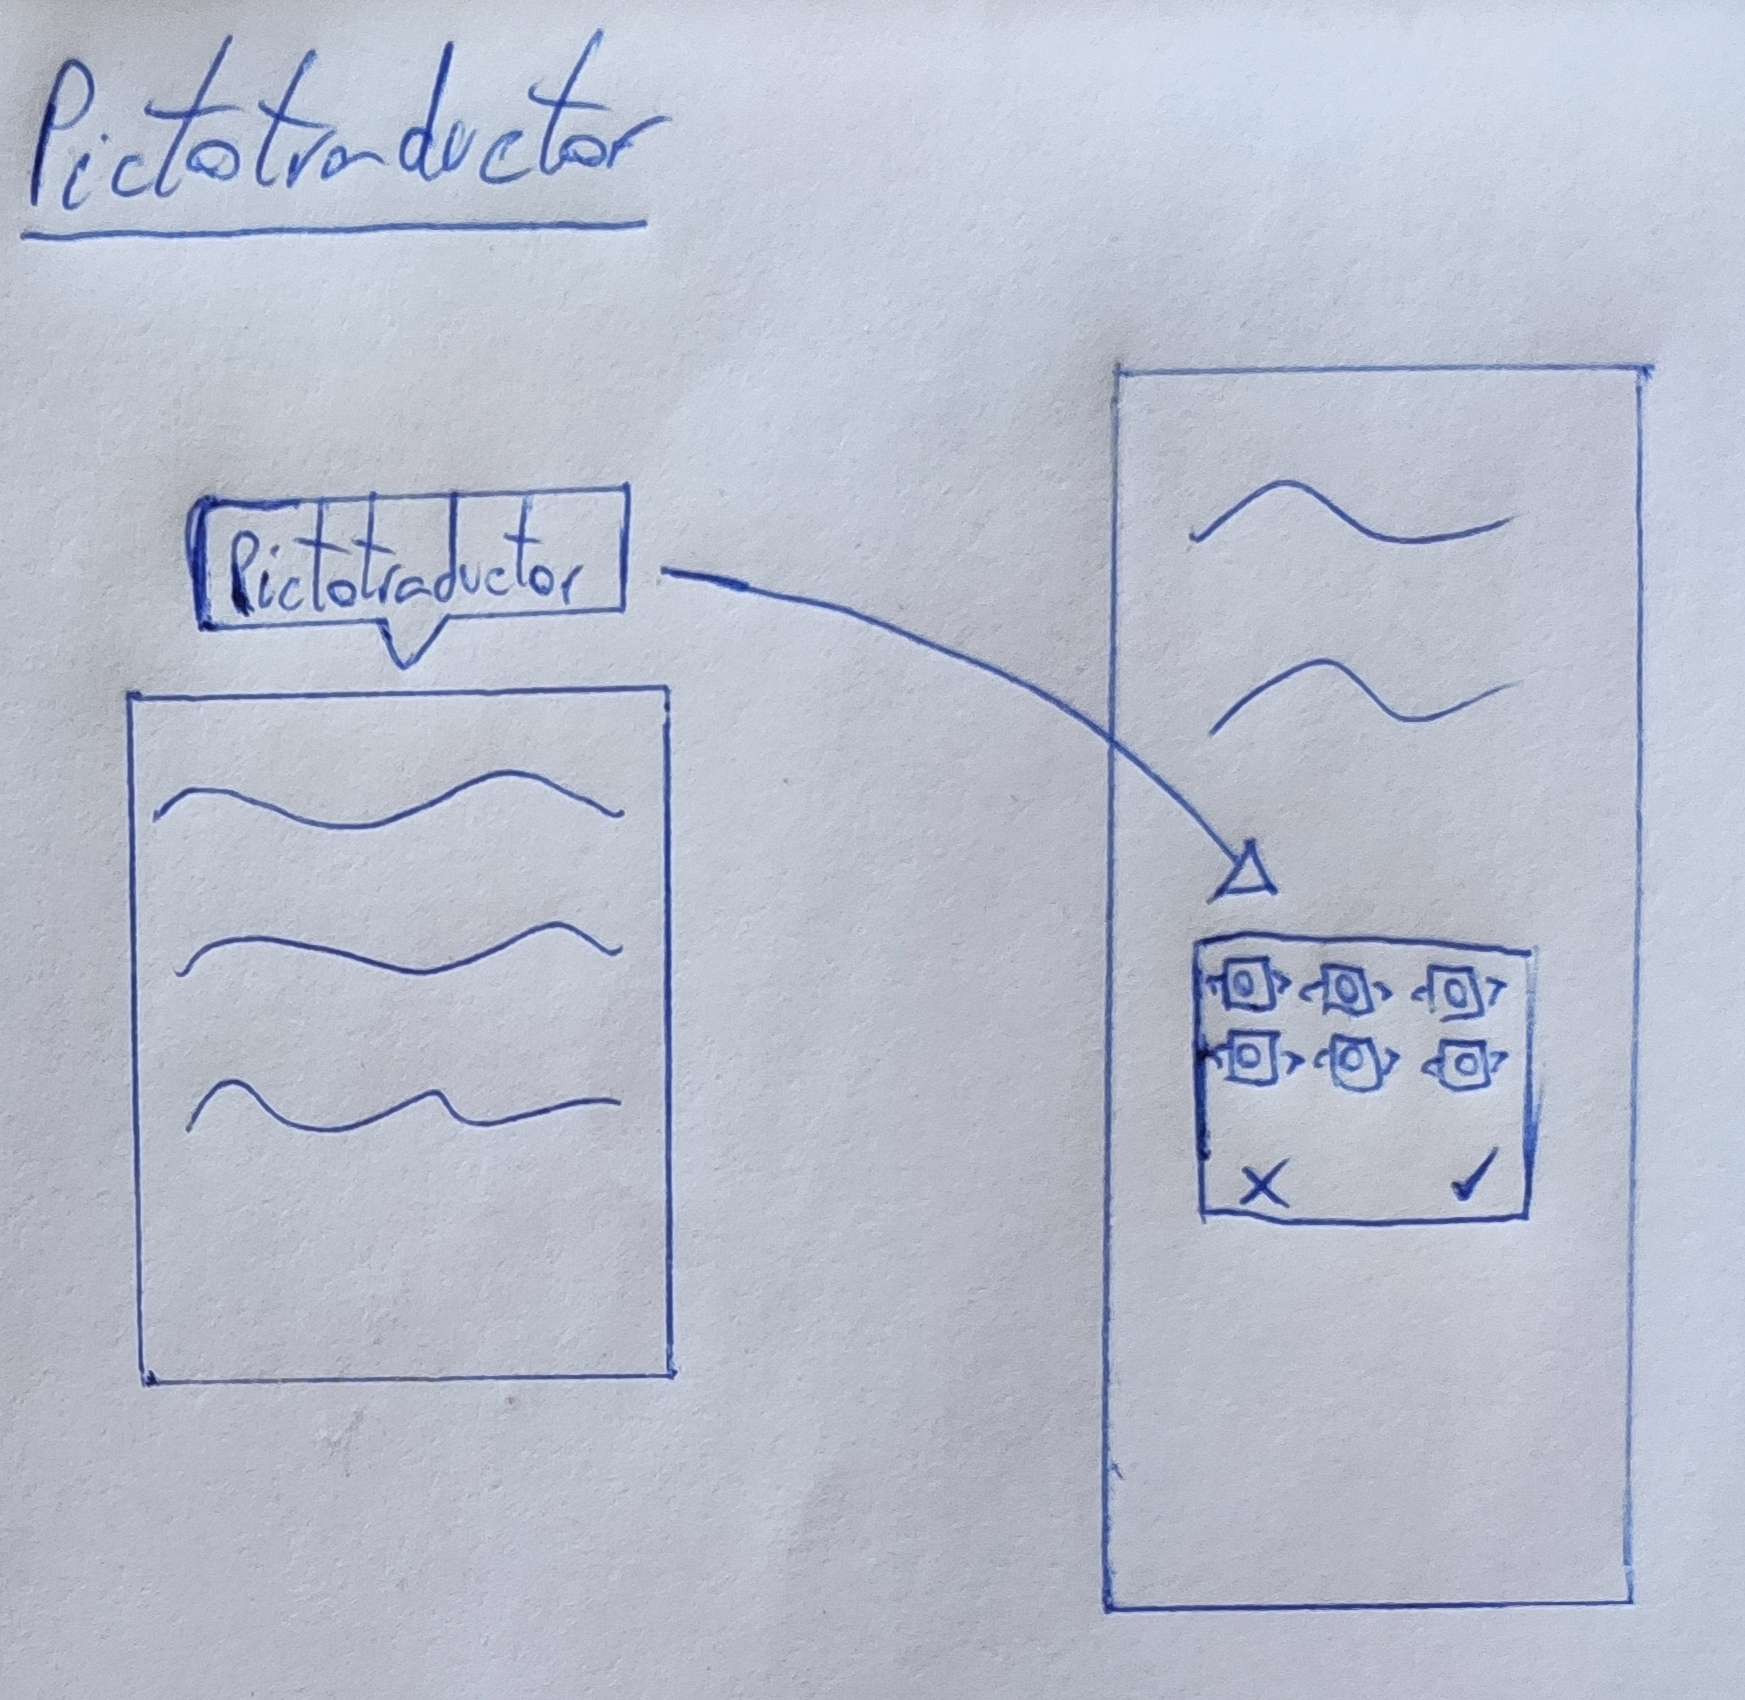
\includegraphics[width=0.5\textwidth]{Diseño/Alvaro/Alvaro04.jpg}
    \caption{Diseño pictotraductor de Álvaro.}
    \label{fig:disenyoAlvaro04}
  \end{subfigure}

  \begin{subfigure}{\textwidth}
    \centering
    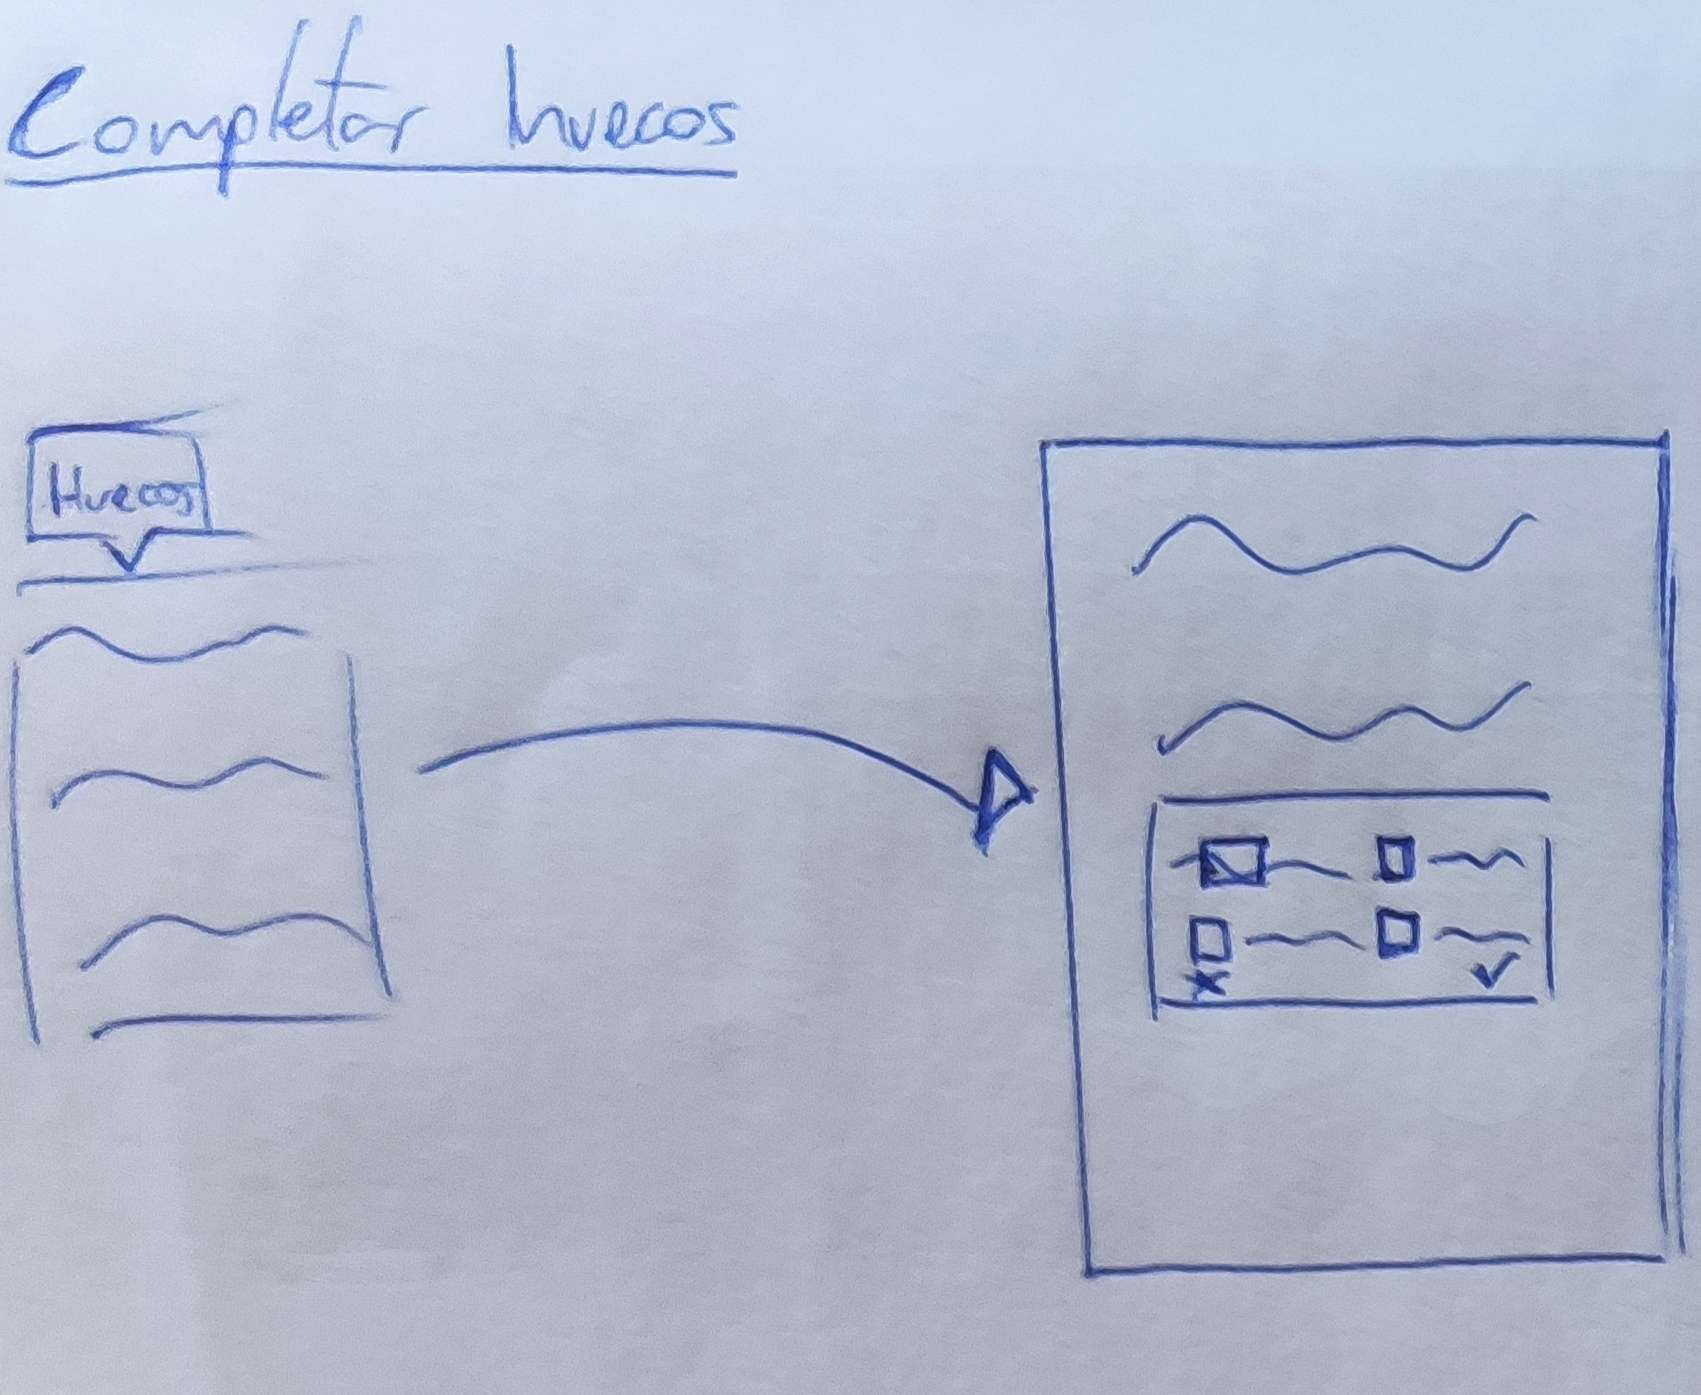
\includegraphics[width=0.5\textwidth]{Diseño/Alvaro/Alvaro05.jpg}
    \caption{Diseño definir huecos de Álvaro.}
    \label{fig:disenyoAlvaro05}
  \end{subfigure}

  \caption{Diseños de Álvaro Gómez Sittima}
  \label{fig:disenyoAlvaro}
\end{figure}


\begin{figure}[ht!]
  \ContinuedFloat

  \begin{subfigure}{\textwidth}
    \centering
    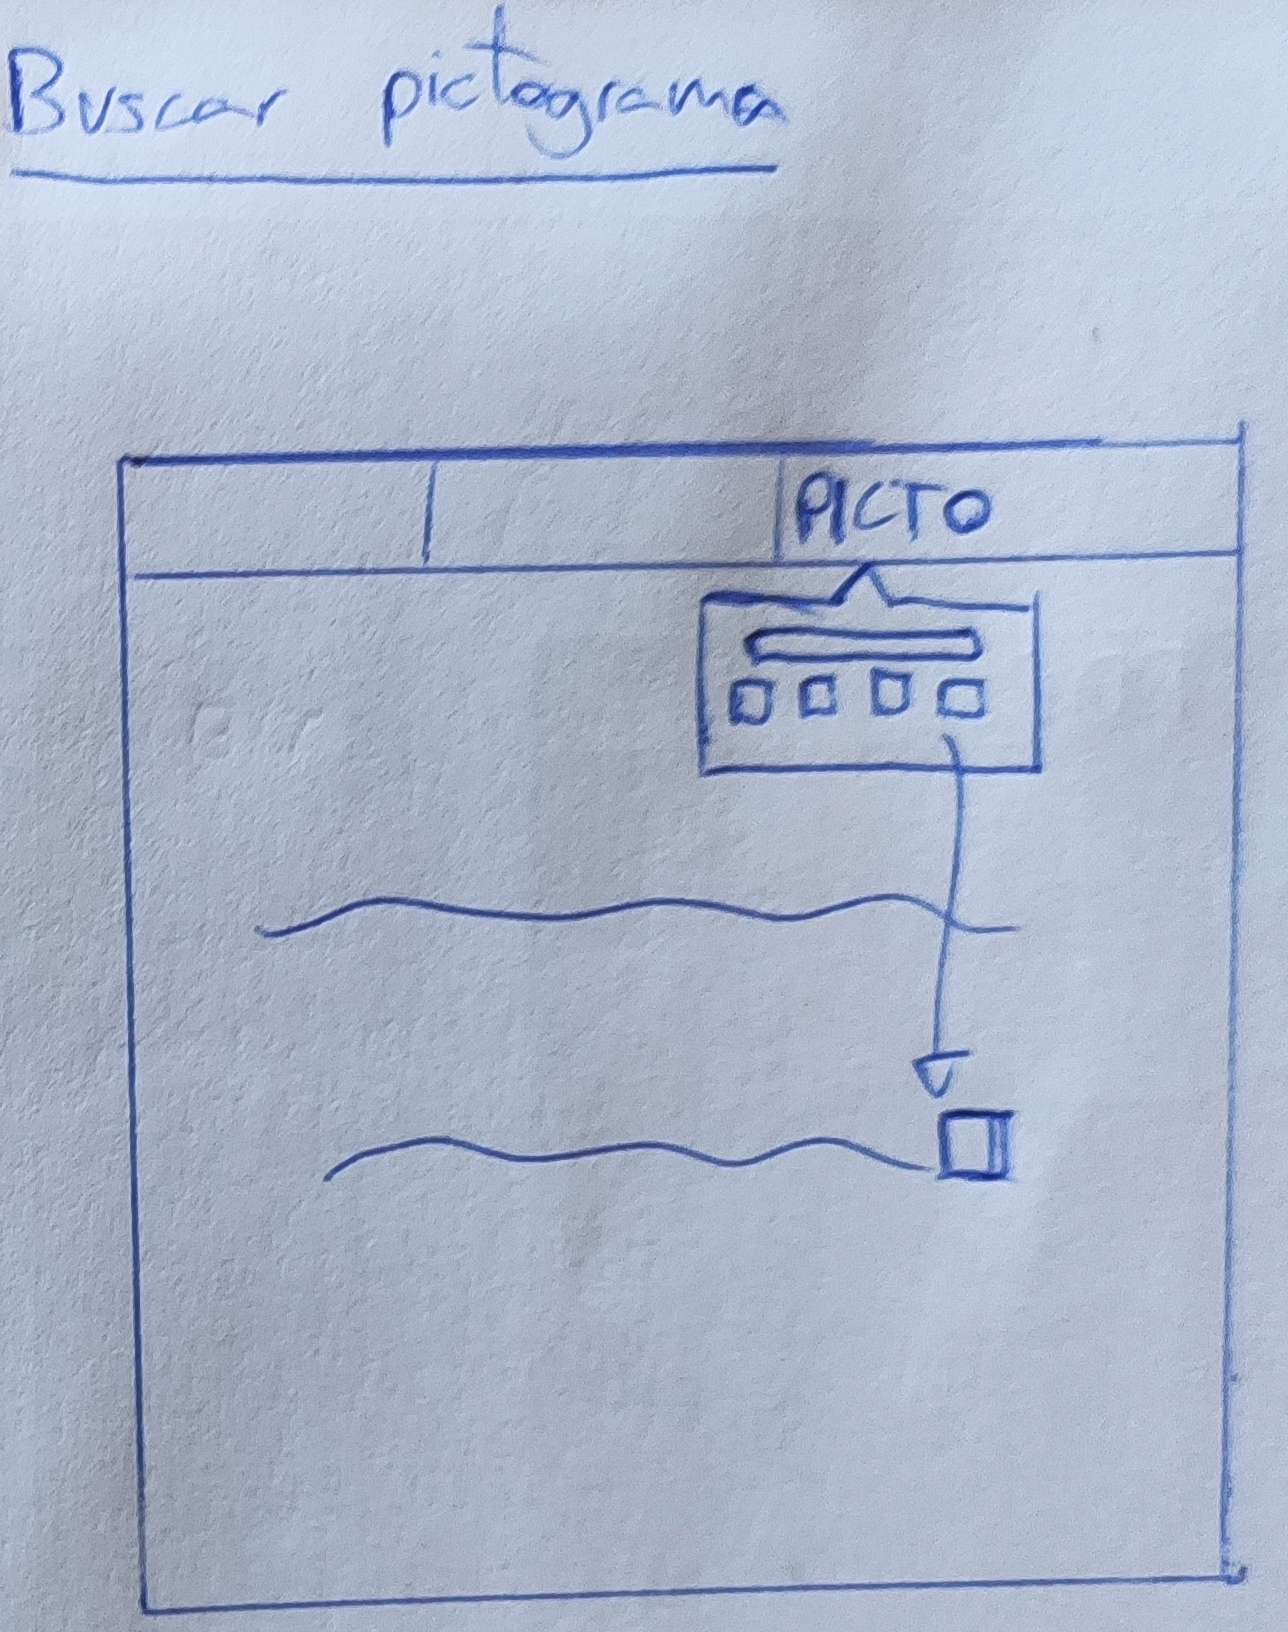
\includegraphics[width=0.6\textwidth]{Diseño/Alvaro/Alvaro06.jpg}
    \caption{Diseño buscar pictogramas de Álvaro.}
    \label{fig:disenyoAlvaro06}
  \end{subfigure}

  \begin{subfigure}{\textwidth}
    \centering
    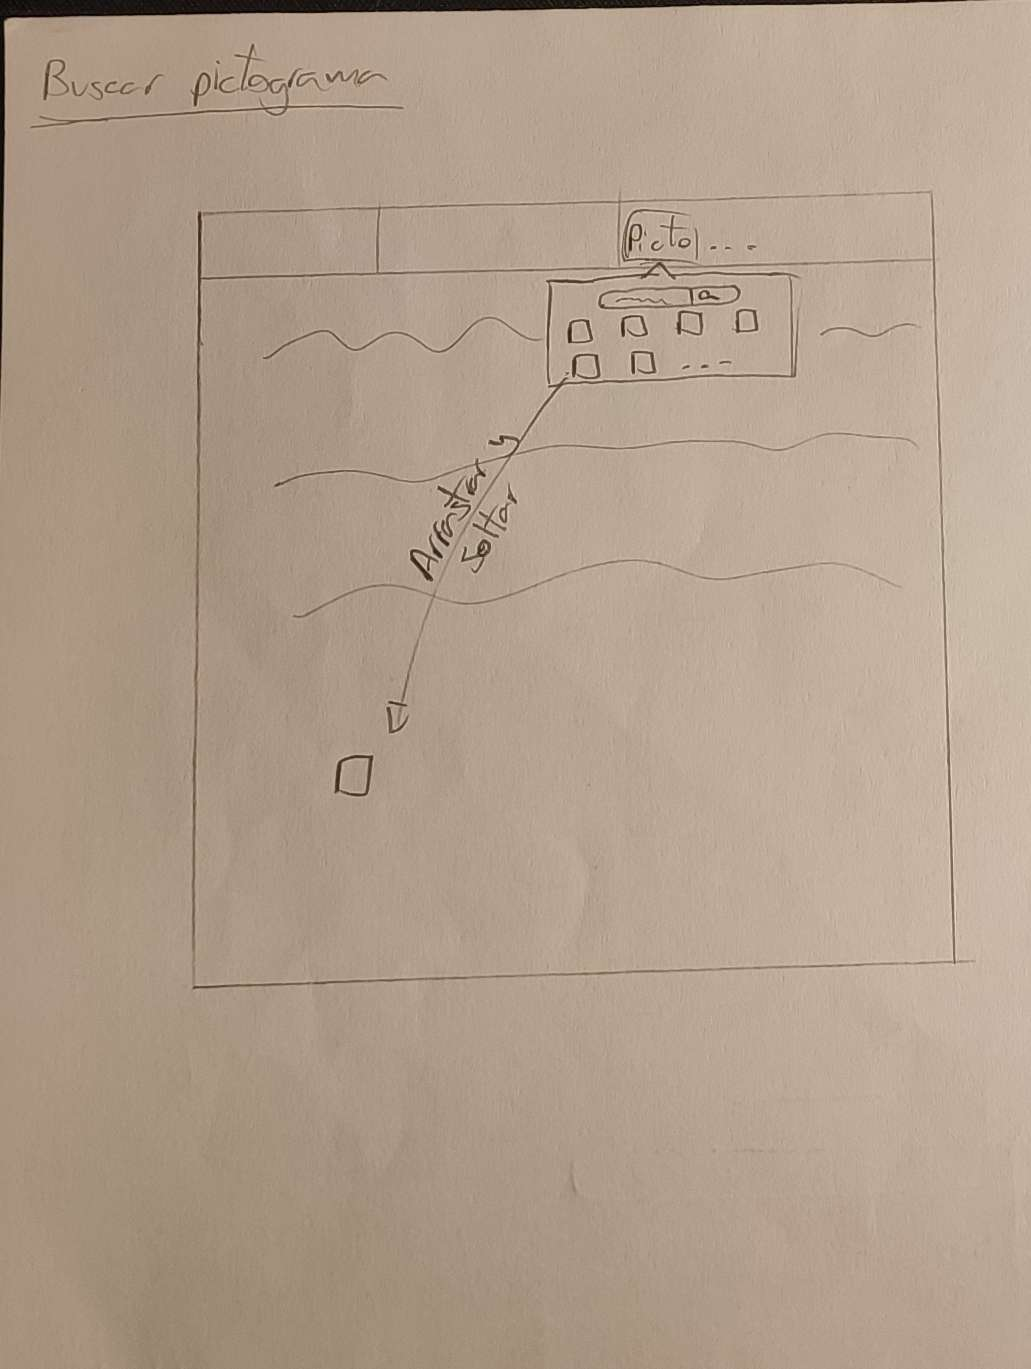
\includegraphics[width=0.6\textwidth]{Diseño/Alvaro/Alvaro07.jpg}
    \caption{Diseño ejercicio de definiciones de Álvaro.}
    \label{fig:disenyoAlvaro07}
  \end{subfigure}

  \caption{Diseños de Álvaro Gómez Sittima}
  \label{fig:disenyoAlvaro}
\end{figure}


\begin{figure}[ht!]
  \section{Dunia Namour Doughani}
  \label{sec:disenyoDunia}
  \begin{subfigure}{\textwidth}
    \centering
    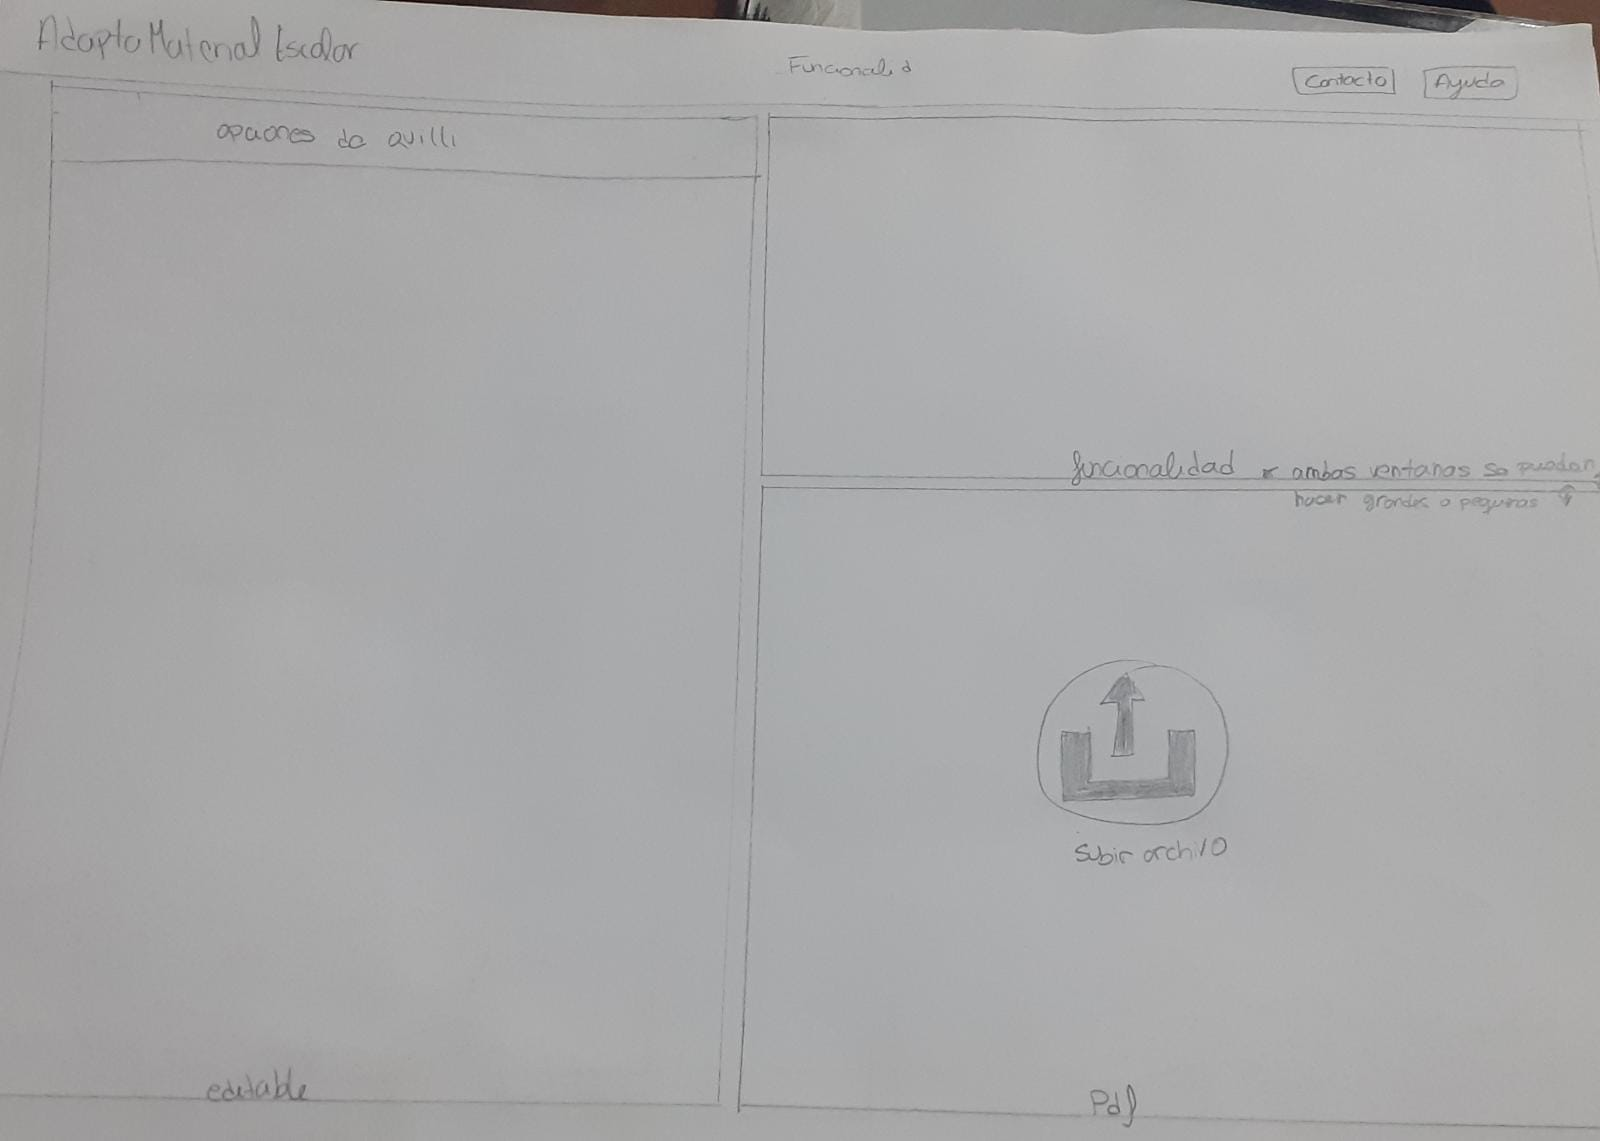
\includegraphics[width=0.6\textwidth]{Diseño/Dunia/principal.jpeg}
    \caption{Diseño pantalla de inicio de Dunia.}
    \label{dunia1}
  \end{subfigure}

  \begin{subfigure}{\textwidth}
    \centering
    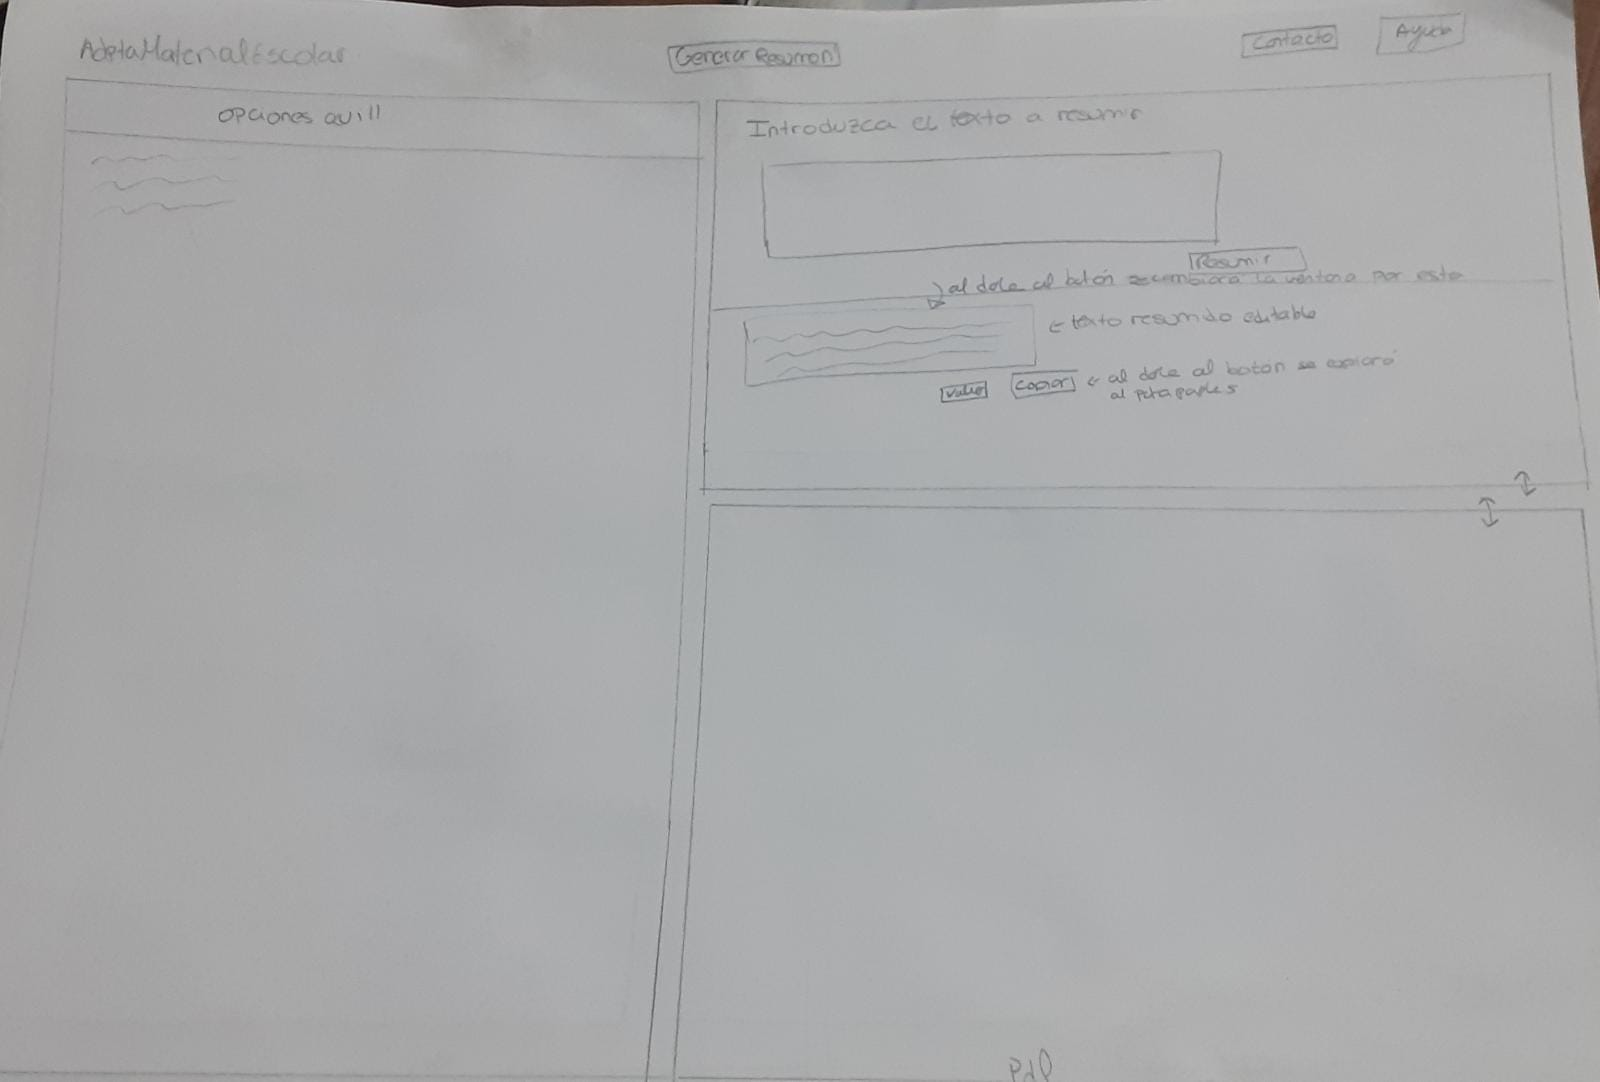
\includegraphics[width=0.6\textwidth]{Diseño/Dunia/resumen.jpeg}
    \caption{Diseño pantalla de generar resumen de Dunia.}
    \label{dunia2}
  \end{subfigure}

  \begin{subfigure}{\textwidth}
    \centering
    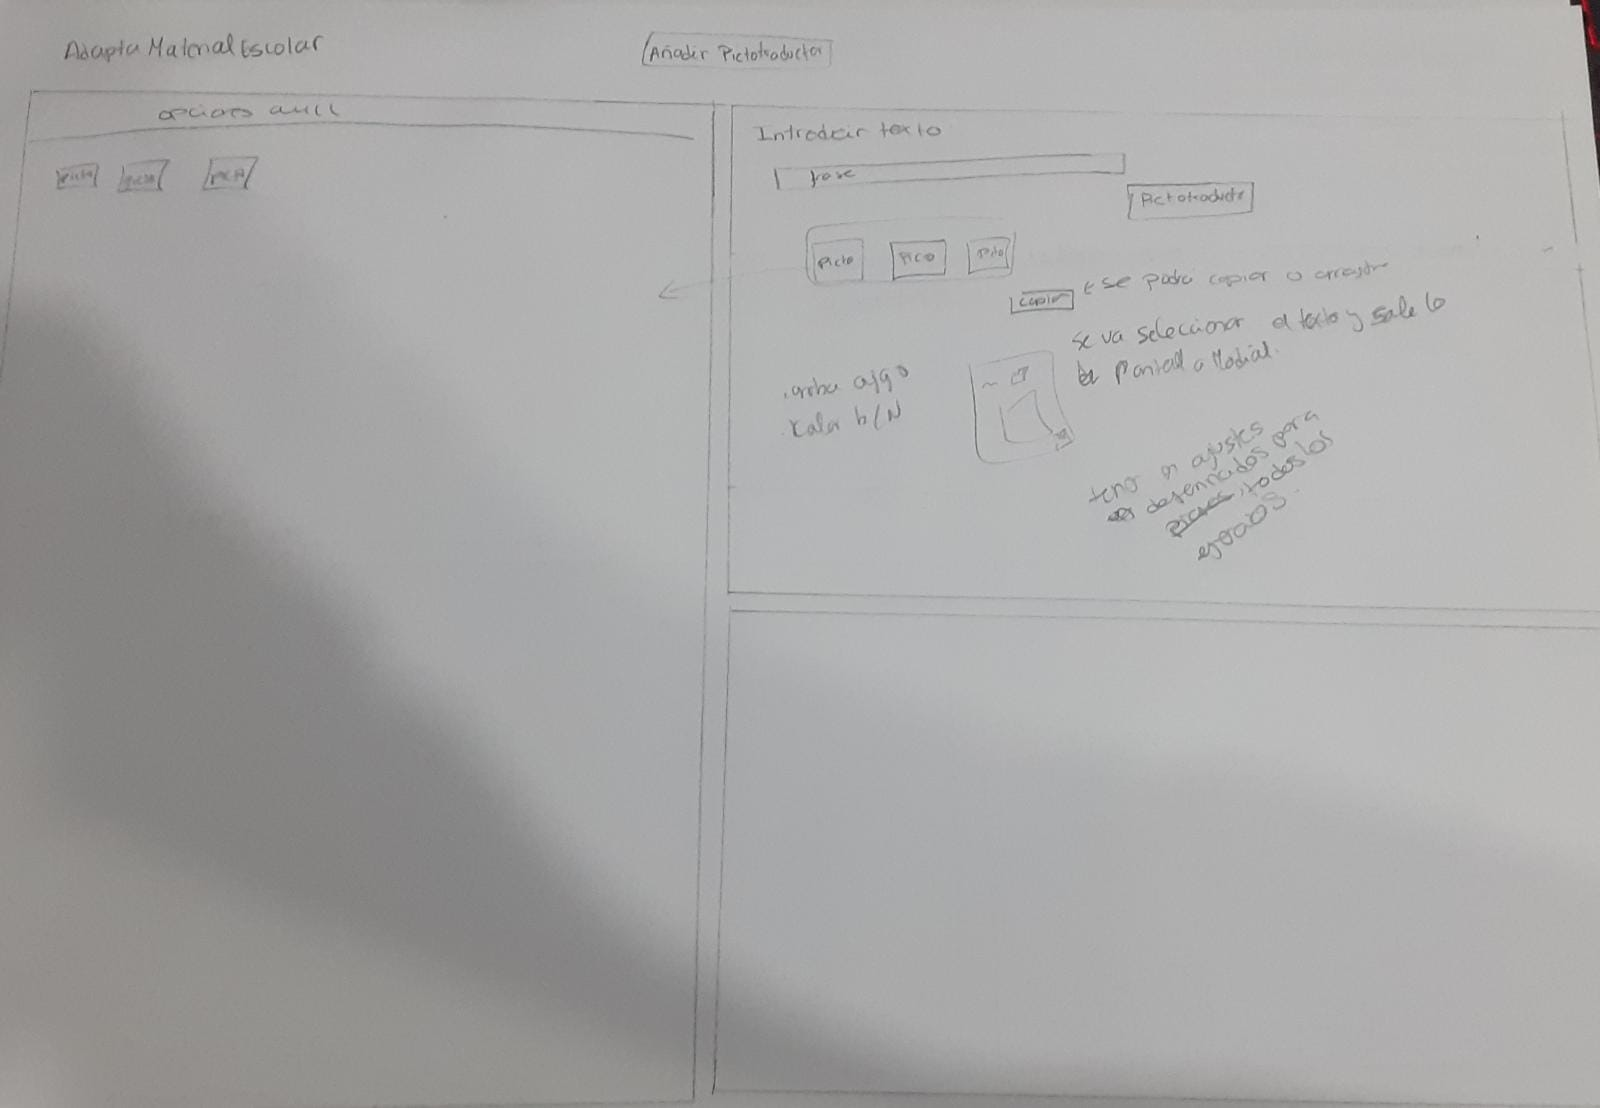
\includegraphics[width=0.6\textwidth]{Diseño/Dunia/picto.jpeg}
    \caption{Diseño de pictotraductor de Dunia.}
    \label{dunia3}
  \end{subfigure}

  \caption{Diseños de Dunia Namour Doughani}
  \label{fig:disenyoDunia}
\end{figure}

\begin{figure}[ht!]
  \ContinuedFloat
  \begin{subfigure}{\textwidth}
    \centering
    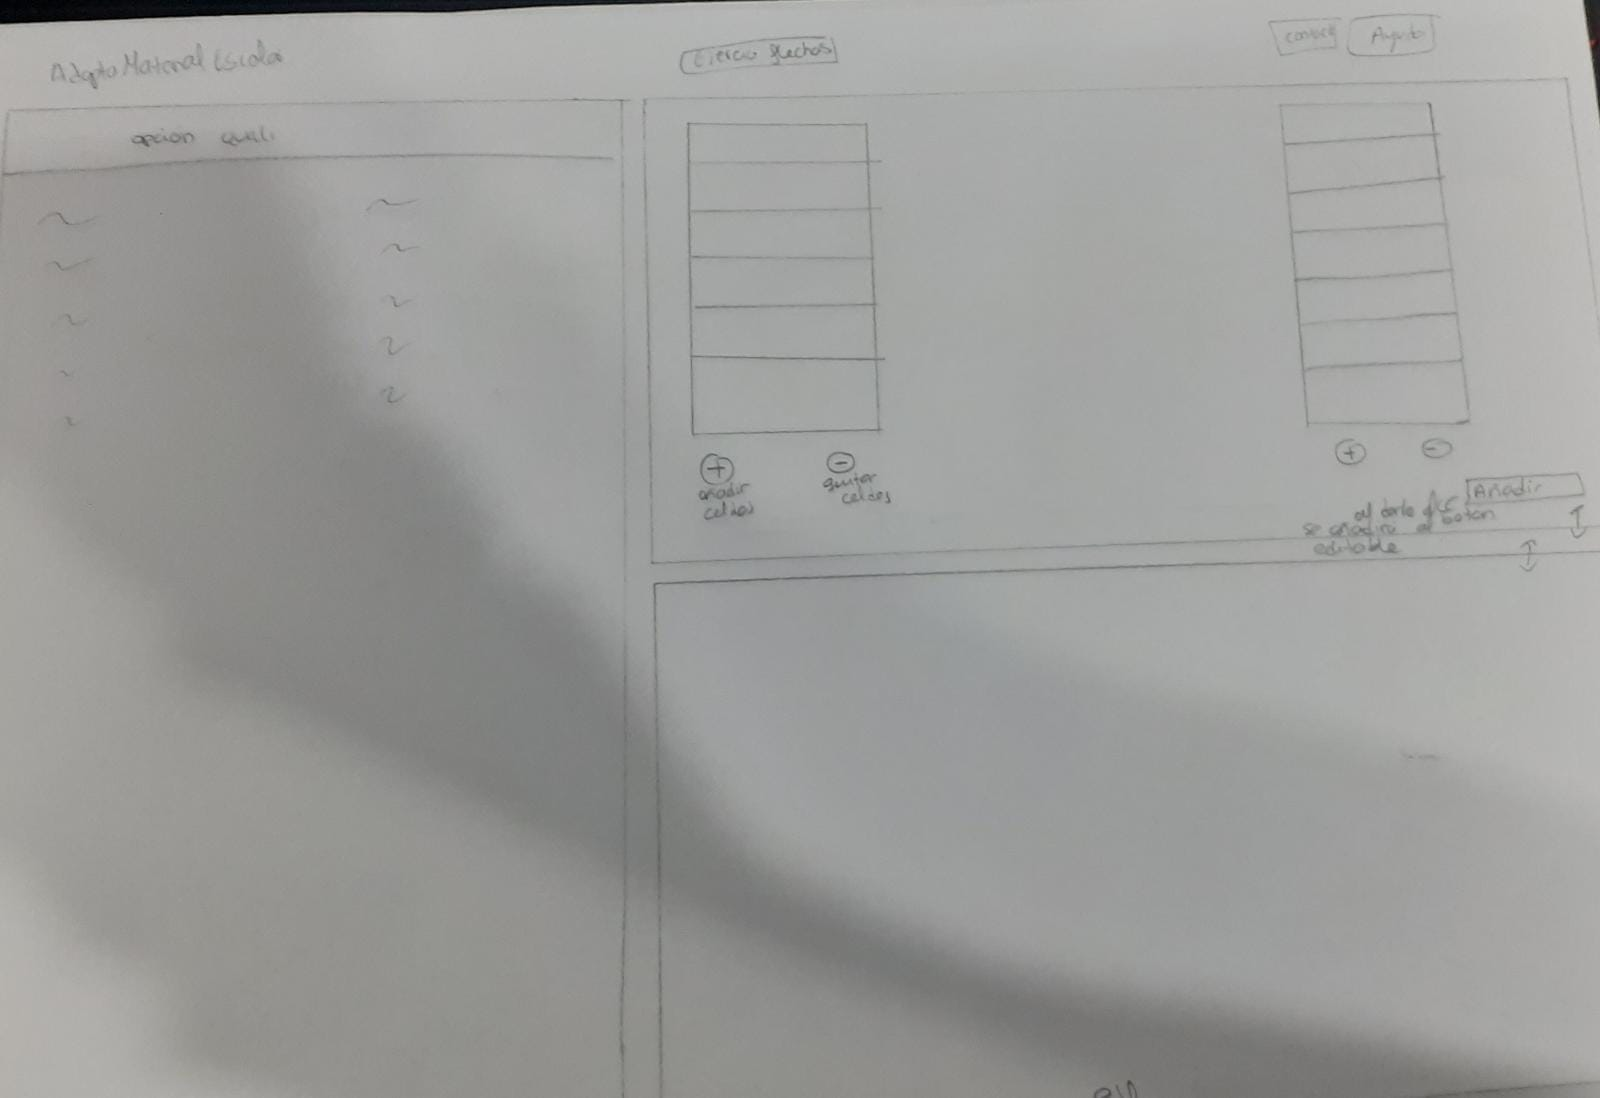
\includegraphics[width=0.7\textwidth]{Diseño/Dunia/flechas.jpeg}
    \caption{Diseño de ejercicios de flechas de Dunia.}
    \label{dunia4}
  \end{subfigure}

  \begin{subfigure}{\textwidth}
    \centering
    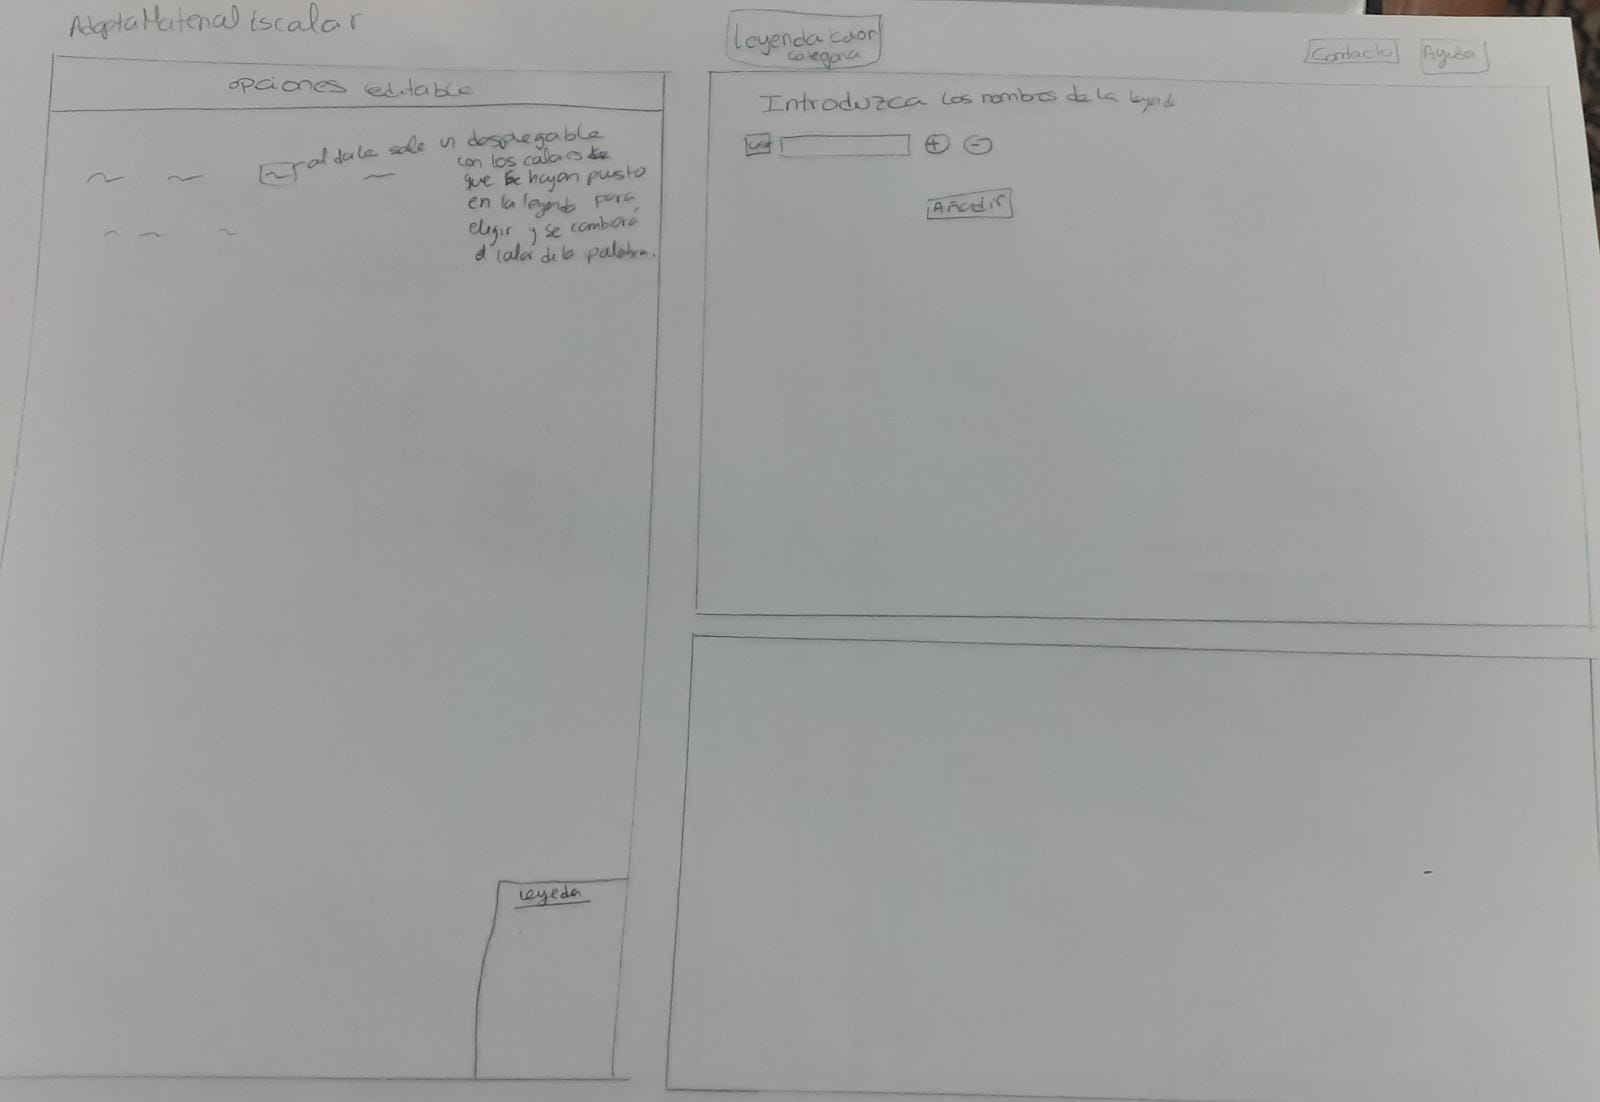
\includegraphics[width=0.7\textwidth]{Diseño/Dunia/leyendaColor.jpeg}
    \caption{Diseño de leyenda de colores de Dunia.}
    \label{dunia5}
  \end{subfigure}

  \begin{subfigure}{\textwidth}
    \centering
    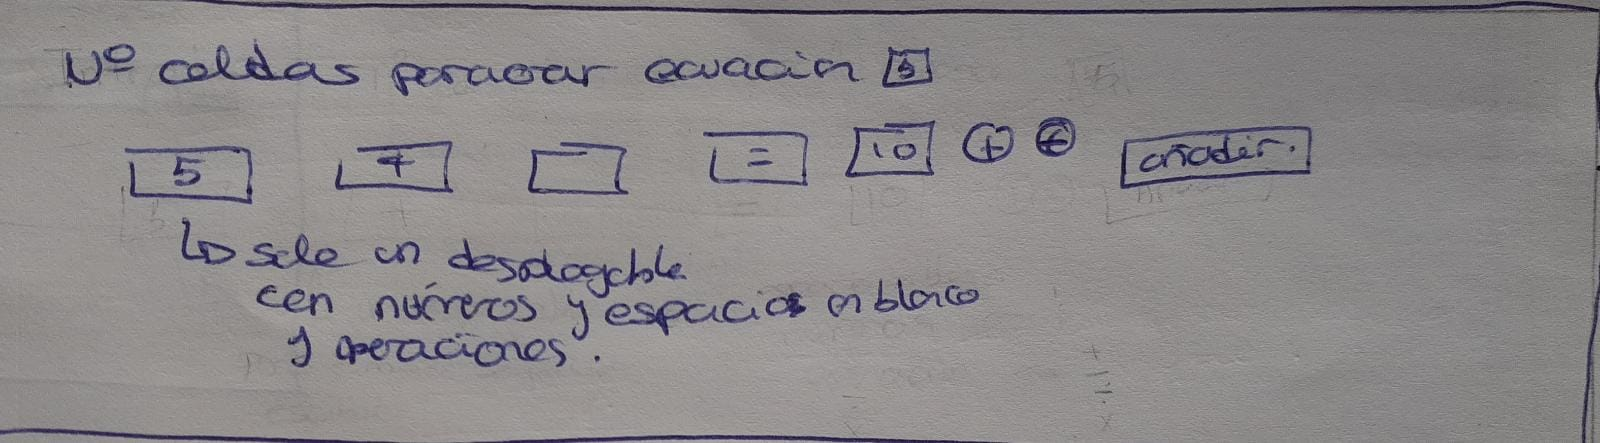
\includegraphics[width=0.7\textwidth]{Diseño/Dunia/hueco.jpeg}
    \caption{Diseño de ejercicios matemáticas de huecos de Dunia.}
    \label{dunia6}
  \end{subfigure}

  \caption{Diseños de Dunia Namour Doughani}
  \label{fig:disenyoDunia}
\end{figure}


\begin{figure}[ht!]
  \section{Alberto Alejandro Rivas Fernandez}
  \label{sec:disenyoAlberto}
  \begin{subfigure}{\textwidth}
    \centering
    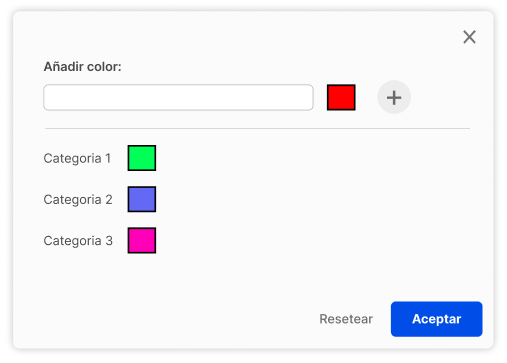
\includegraphics[width=0.6\textwidth]{Diseño/Alberto/Capture01.PNG}
    \caption{Diseño de leyenda de colores de Alberto.}
    \label{Alberto1}
  \end{subfigure}

  \begin{subfigure}{\textwidth}
    \centering
    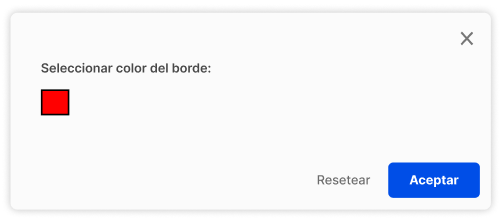
\includegraphics[width=0.6\textwidth]{Diseño/Alberto/Capture02.PNG}
    \caption{Diseño de leyenda de colores por asignatura de Alberto.}
    \label{Alberto2}
  \end{subfigure}

  \begin{subfigure}{\textwidth}
    \centering
    
\includegraphics[width=0.6\textwidth]{Diseño/Alberto/Capture03.PNG}
    \caption{Diseño de cuatrícula de Alberto.}
    \label{Alberto3}
  \end{subfigure}

  \caption{Diseños de Alberto Alejandro Rivas Fernandez}
  \label{fig:disenyoAlberto}
\end{figure}

\begin{figure}[ht!]
  \ContinuedFloat
  \begin{subfigure}{\textwidth}
    \centering
    
\includegraphics[width=0.6\textwidth]{Diseño/Alberto/Capture04.PNG}
    \caption{Diseño de doble pauta de Alberto.}
    \label{Alberto4}
  \end{subfigure}

  \begin{subfigure}{\textwidth}
    \centering
    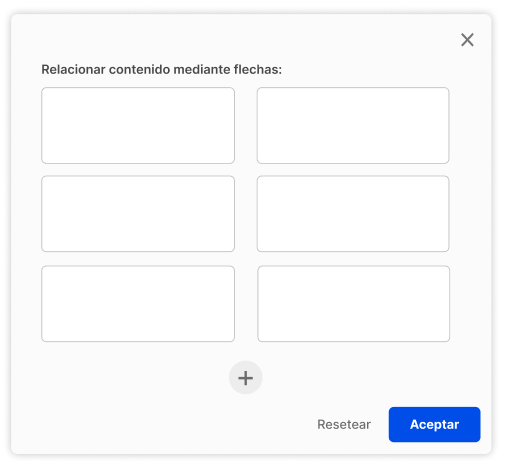
\includegraphics[width=0.6\textwidth]{Diseño/Alberto/Capture05.PNG}
    \caption{Diseño de ejercicio de flechas de Alberto.}
    \label{Alberto5}
  \end{subfigure}

  \begin{subfigure}{\textwidth}
    \centering
    
\includegraphics[width=0.6\textwidth]{Diseño/Alberto/Capture06.PNG}
    \caption{Diseño de ejercicios de matemáticas con huecos de Alberto.}
    \label{Alberto6}
  \end{subfigure}

  \caption{Diseños de Alberto Alejandro Rivas Fernandez}
  \label{fig:disenyoAlberto}
\end{figure}


\begin{figure}[ht!]
  \ContinuedFloat
  \begin{subfigure}{\textwidth}
    \centering
    
\includegraphics[width=0.6\textwidth]{Diseño/Alberto/Capture07.PNG}
    \caption{Diseño de ejercicios de espacios para dibujar de Alberto.}
    \label{Alberto7}
  \end{subfigure}

  \begin{subfigure}{\textwidth}
    \centering
    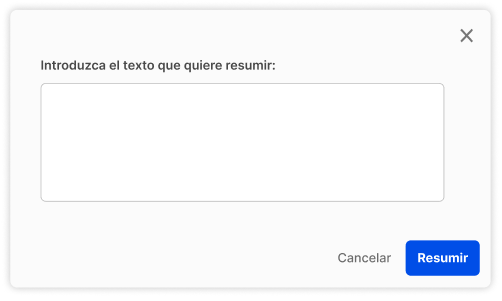
\includegraphics[width=0.6\textwidth]{Diseño/Alberto/Capture08.PNG}
    \caption{Diseño de añadir resumen de Alberto.}
    \label{Alberto8}
  \end{subfigure}

  \begin{subfigure}{\textwidth}
    \centering
    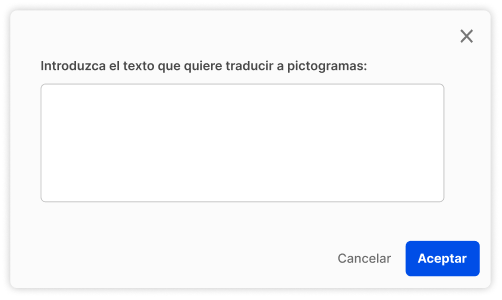
\includegraphics[width=0.6\textwidth]{Diseño/Alberto/Capture10.PNG}
    \caption{Diseño de pictotraductor de Alberto.}
    \label{Alberto10}
  \end{subfigure}

  \caption{Diseños de Alberto Alejandro Rivas Fernandez}
  \label{fig:disenyoAlberto}
\end{figure}

\begin{figure}[ht!]
  \ContinuedFloat
  \begin{subfigure}{\textwidth}
    \centering
    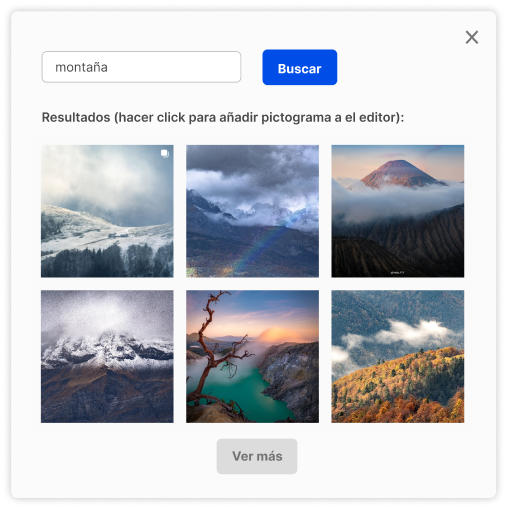
\includegraphics[width=0.6\textwidth]{Diseño/Alberto/Capture12.PNG}
    \caption{Diseño de buscar pictogramas de Alberto.}
    \label{Alberto12}
  \end{subfigure}

  \begin{subfigure}{\textwidth}
    \centering
    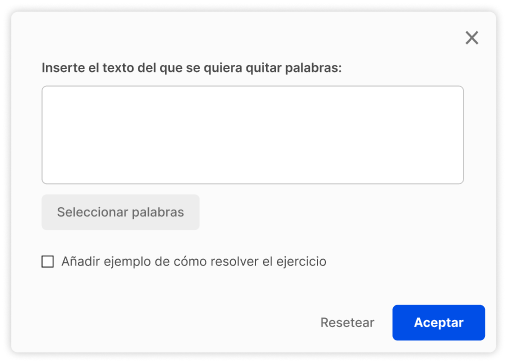
\includegraphics[width=0.6\textwidth]{Diseño/Alberto/Capture13.PNG}
    \caption{Diseño de ejercicios con huecos de Alberto.}
    \label{Alberto13}
  \end{subfigure}

  \begin{subfigure}{\textwidth}
    \centering
    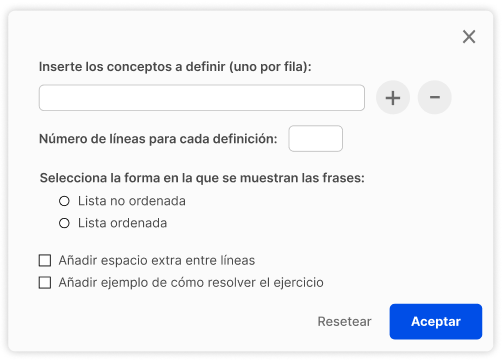
\includegraphics[width=0.6\textwidth]{Diseño/Alberto/Capture14.PNG}
    \caption{Diseño de ejercicios de definiciones de Alberto.}
    \label{Alberto14}
  \end{subfigure}

  \caption{Diseños de Alberto Alejandro Rivas Fernandez}
  \label{fig:disenyoAlberto}
\end{figure}


\begin{figure}[ht!]
  \ContinuedFloat
  \begin{subfigure}{\textwidth}
    \centering
    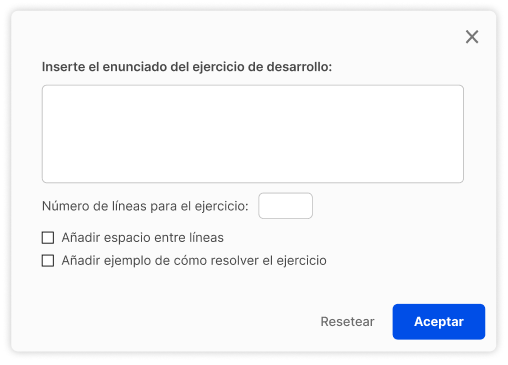
\includegraphics[width=0.6\textwidth]{Diseño/Alberto/Capture15.PNG}
    \caption{Diseño de ejercicios de desarrollo de Alberto.}
    \label{Alberto15}
  \end{subfigure}

  \begin{subfigure}{\textwidth}
    \centering
    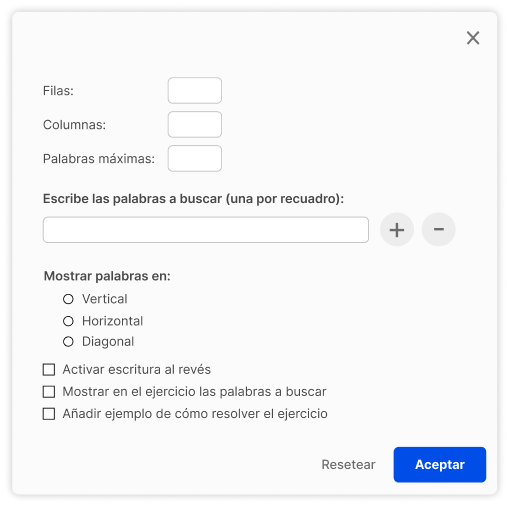
\includegraphics[width=0.6\textwidth]{Diseño/Alberto/Capture16.PNG}
    \caption{Diseño de ejercicios de sopa de letras de Alberto.}
    \label{Alberto16}
  \end{subfigure}

  \begin{subfigure}{\textwidth}
    \centering
    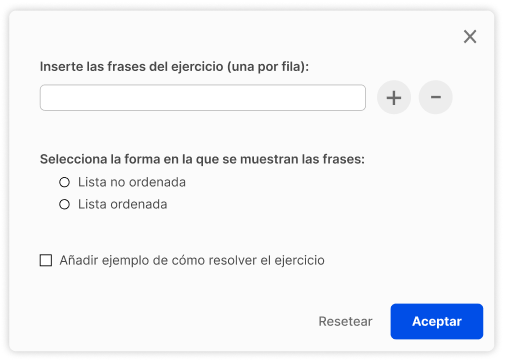
\includegraphics[width=0.6\textwidth]{Diseño/Alberto/Capture17.PNG}
    \caption{Diseño de ejercicios de verdadero y falso de Alberto.}
    \label{Alberto17}
  \end{subfigure}

  \caption{Diseños de Alberto Alejandro Rivas Fernandez}
  \label{fig:disenyoAlberto}
\end{figure}

\begin{figure}[ht!]
  \ContinuedFloat
  \begin{subfigure}{\textwidth}
    \centering
    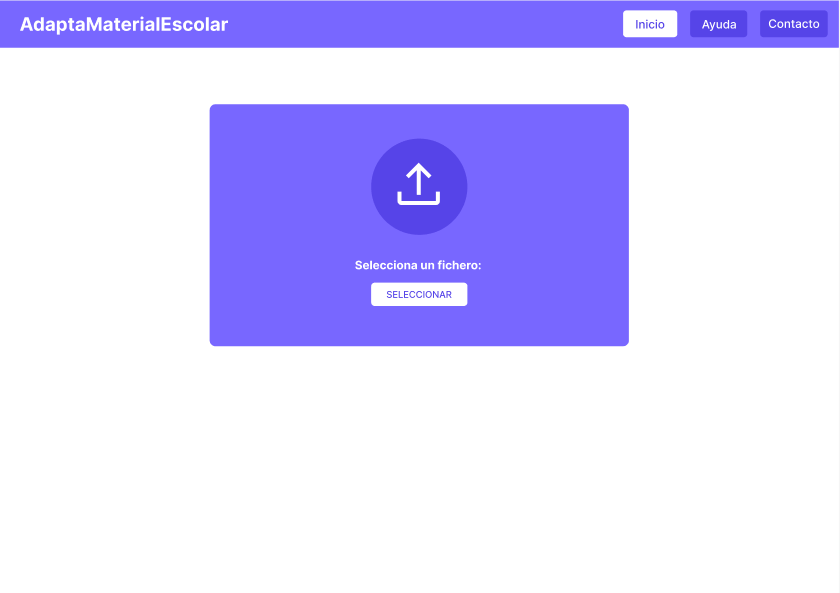
\includegraphics[width=0.6\textwidth]{Diseño/Alberto/PaginaPrincipal1.PNG}
    \caption{Diseño página principal de Alberto.}
    \label{AlbertoPaginaPrincipal1}
  \end{subfigure}

  \begin{subfigure}{\textwidth}
    \centering
    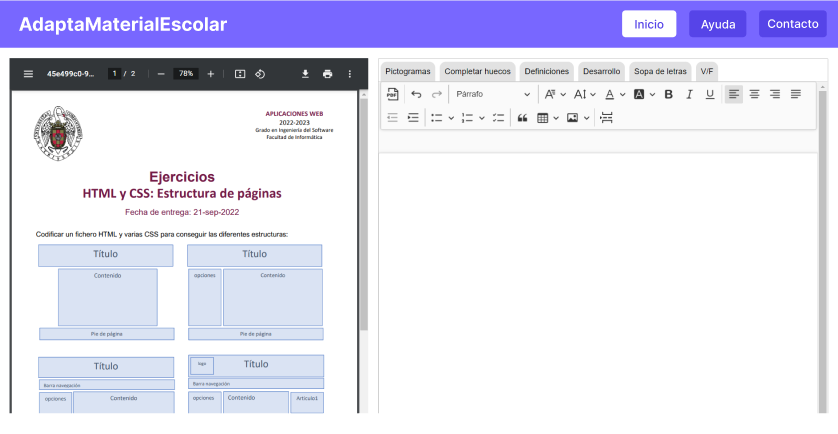
\includegraphics[width=0.6\textwidth]{Diseño/Alberto/PaginaPrincipal2.PNG}
    \caption{Diseño página principal de Alberto.}
    \label{AlbertoPaginaPrincipal2}
  \end{subfigure}

  \caption{Diseños de Alberto Alejandro Rivas Fernandez}
  \label{fig:disenyoAlberto}
\end{figure}


\begin{figure}[ht!]
  \section{Johan Sebastian Salvatierra Gutierrez}
  \label{sec:disenyoJohan}
  \begin{subfigure}{\textwidth}
    \centering
    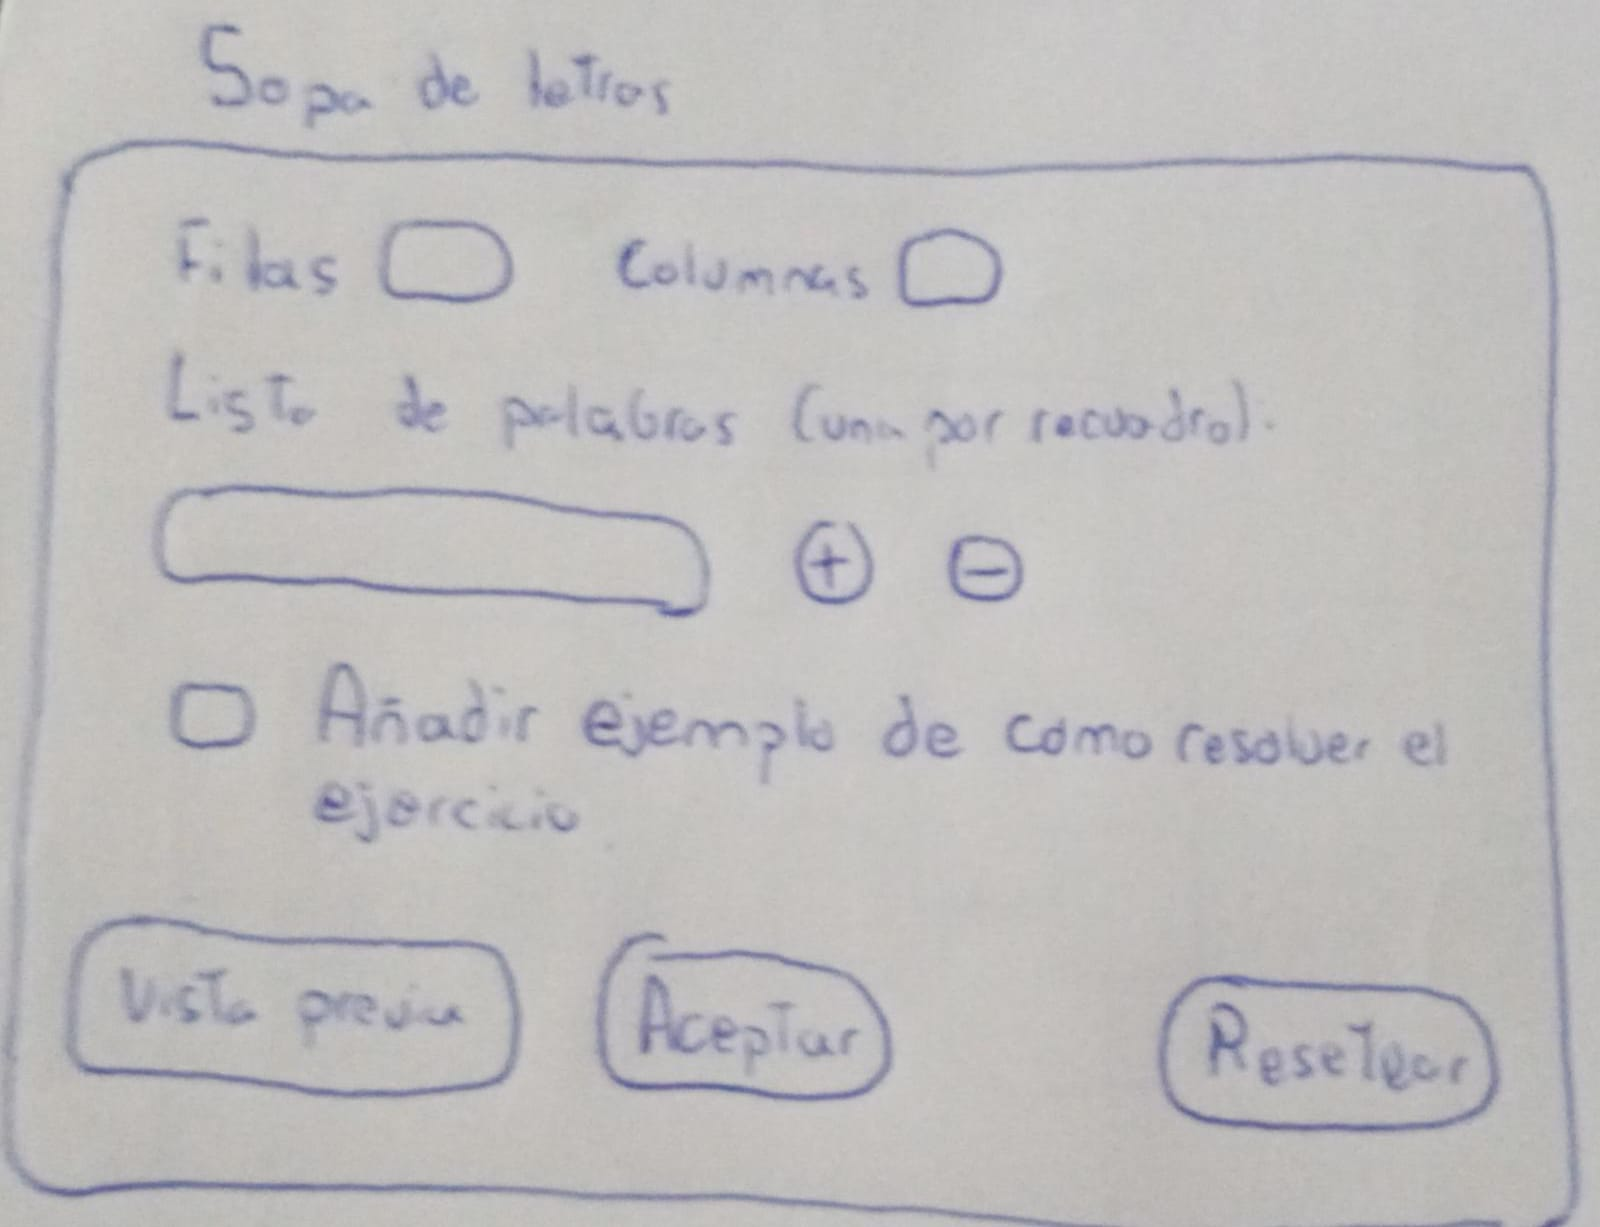
\includegraphics[width=0.6\textwidth]{Diseño/Johan/Johan1.jpeg}
    \caption{Diseño de sopa de letras.}
    \label{Johan1}
  \end{subfigure}

  \begin{subfigure}{\textwidth}
    \centering
    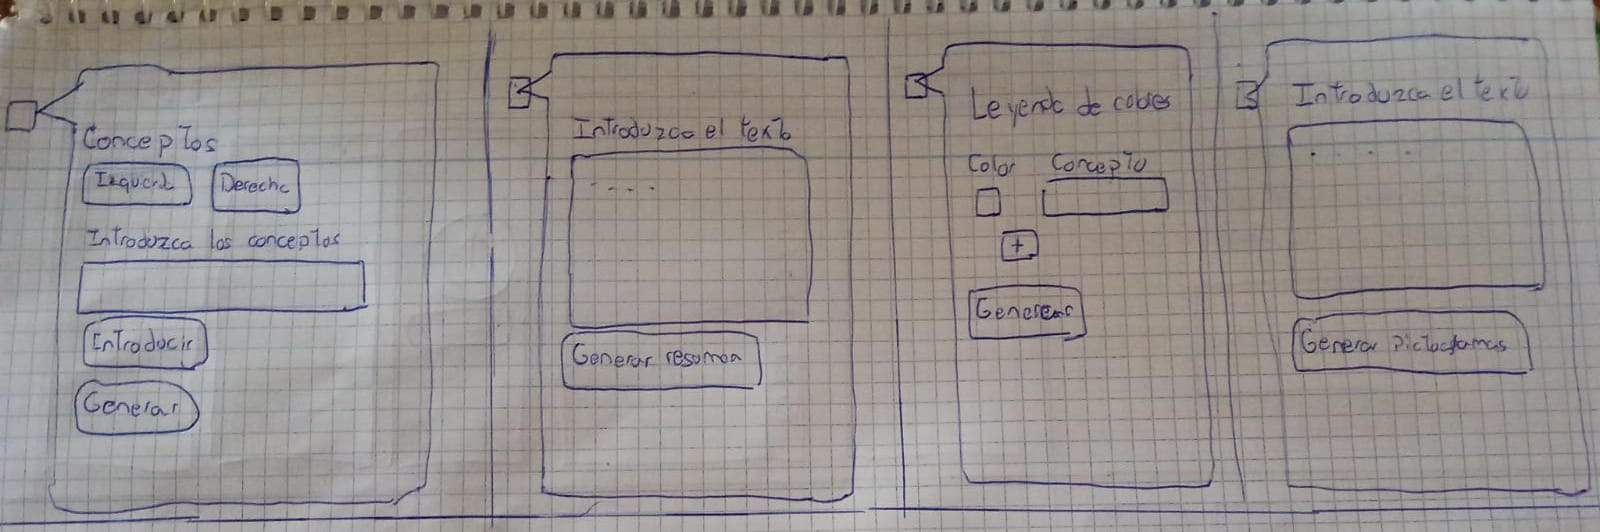
\includegraphics[width=0.6\textwidth]{Diseño/Johan/Johan2.jpeg}
    \caption{Diseño de leyenda de Johan.}
    \label{Johan2}
  \end{subfigure}

  \begin{subfigure}{\textwidth}
    \centering
    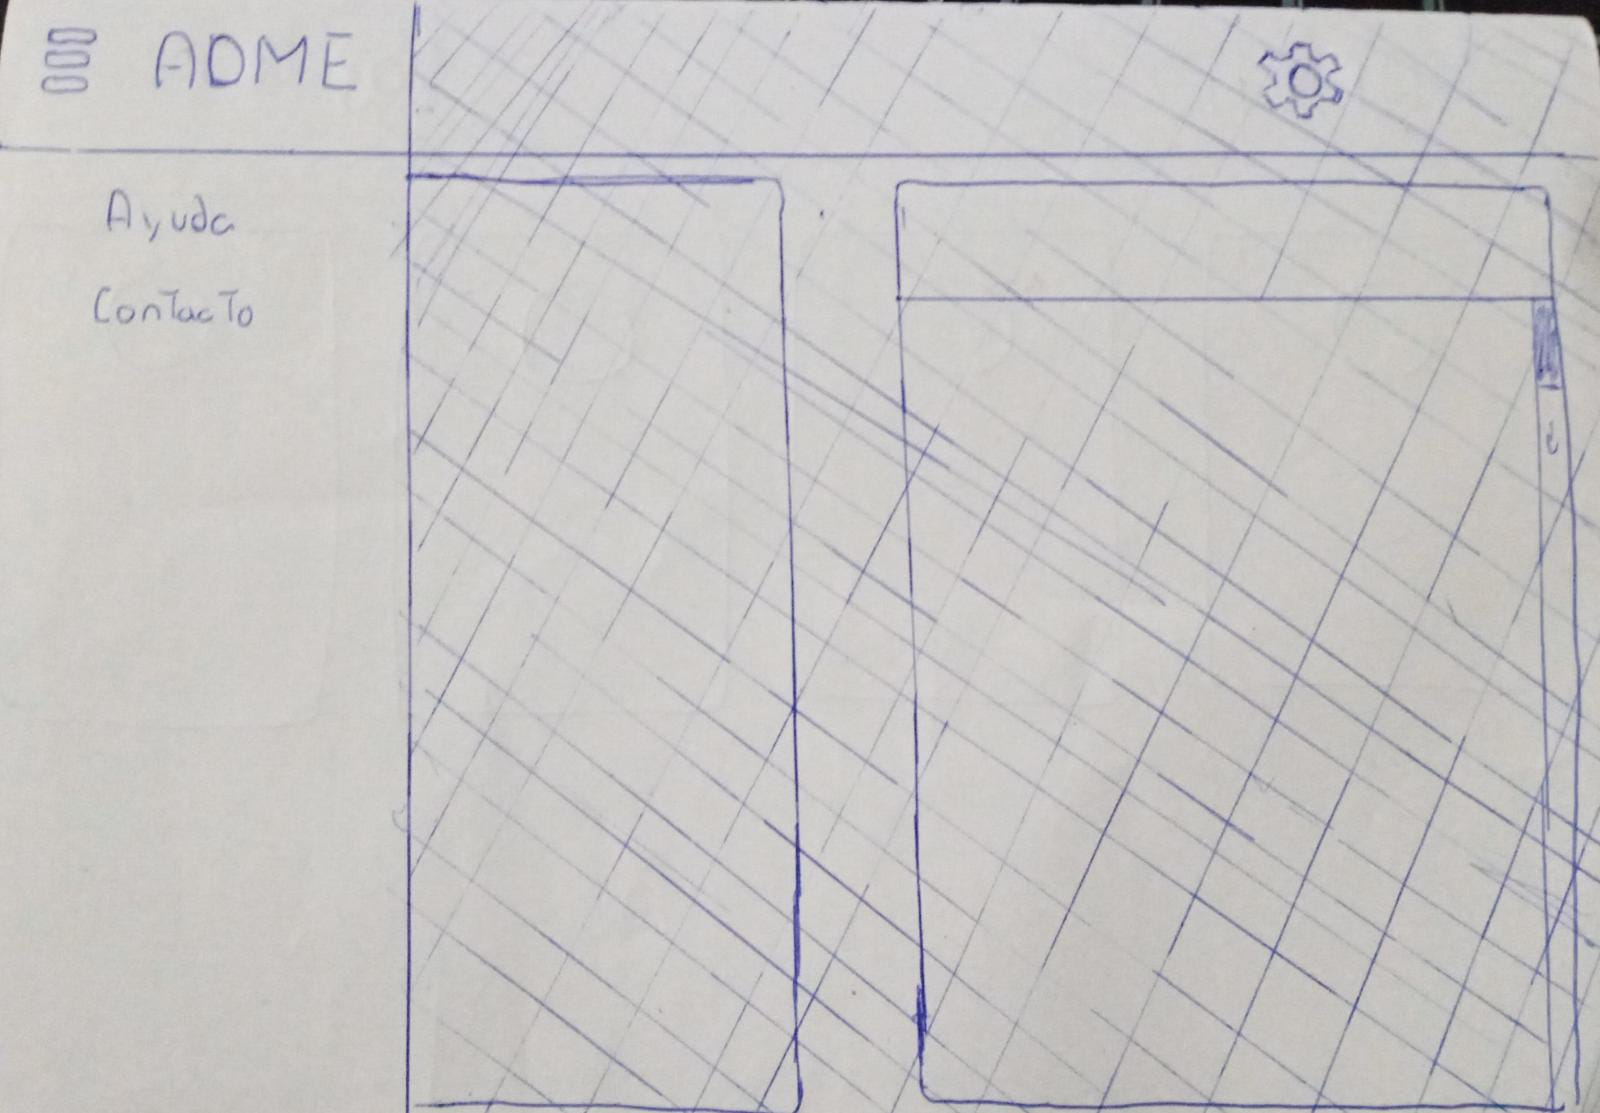
\includegraphics[width=0.6\textwidth]{Diseño/Johan/Johan3.jpeg}
    \caption{Diseño de ejercicios de flechas de Johan.}
    \label{Johan3}
  \end{subfigure}

  \caption{Diseños de Johan Sebastian Salvatierra Gutierrez}
  \label{fig:disenyoJohan}
\end{figure}

\begin{figure}[ht!]
  \ContinuedFloat
  \begin{subfigure}{\textwidth}
    \centering
    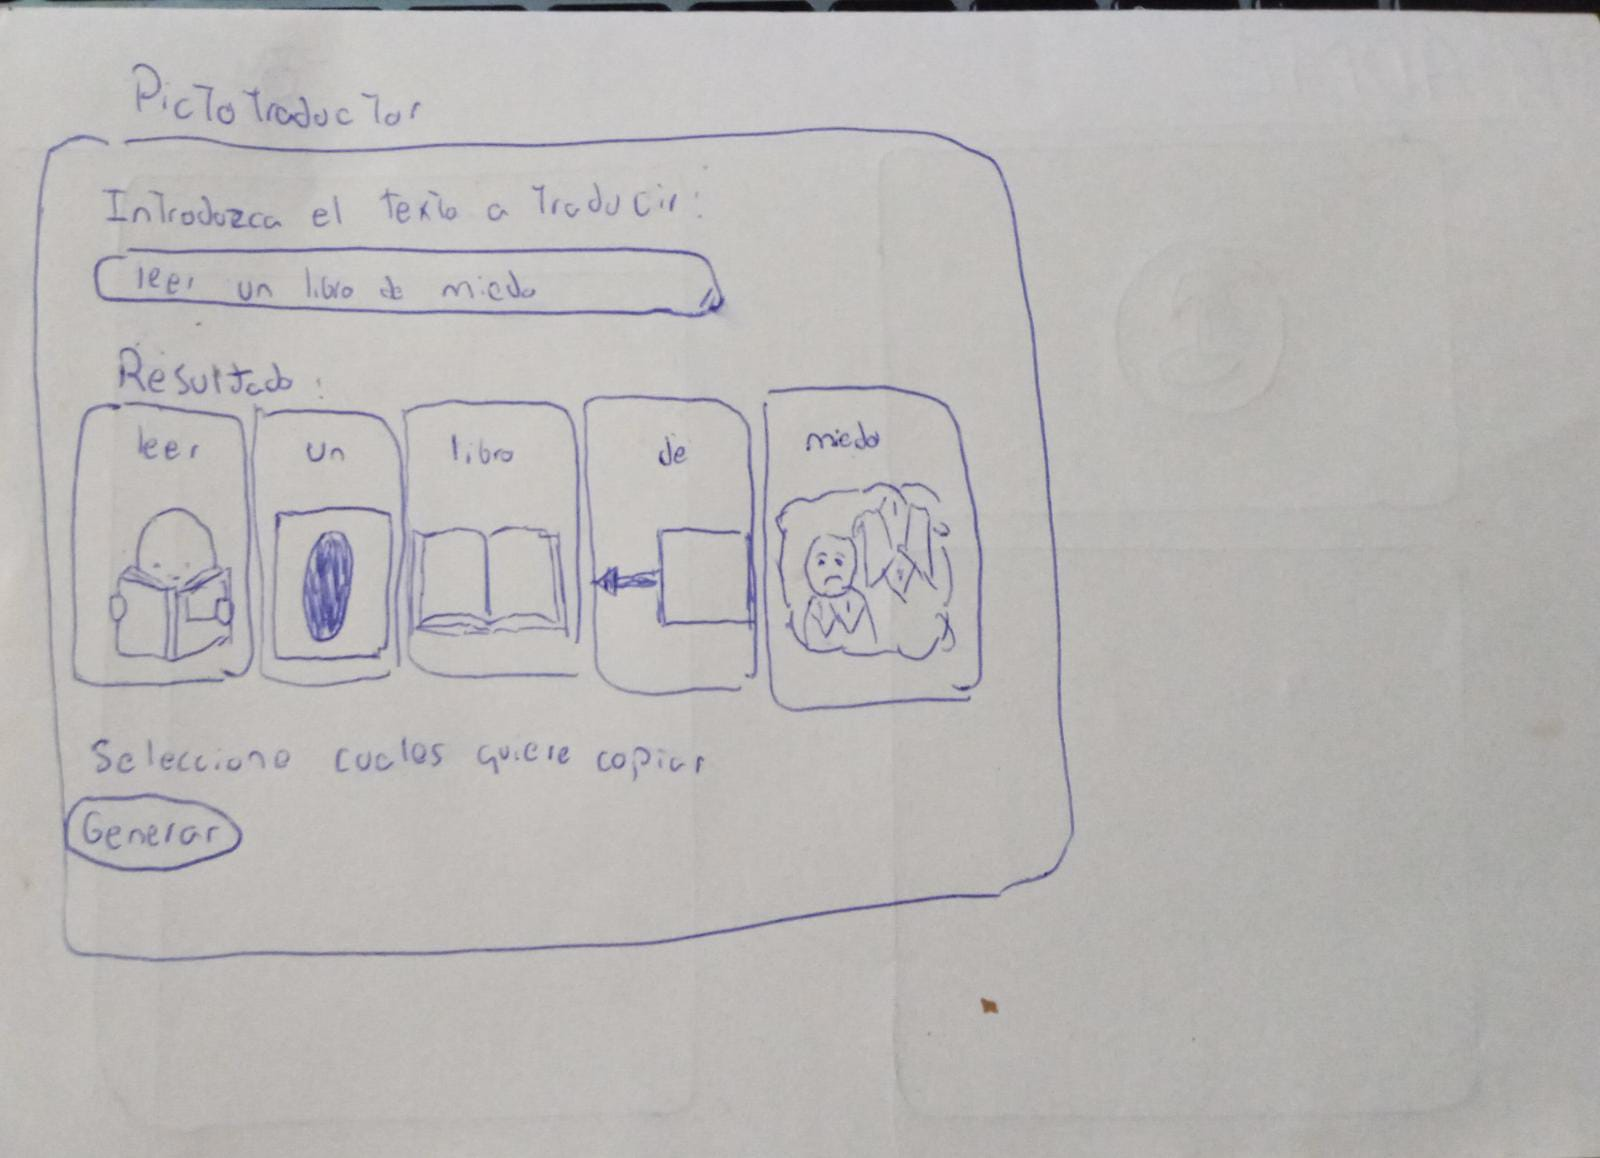
\includegraphics[width=0.6\textwidth]{Diseño/Johan/Johan4.jpeg}
    \caption{Diseño de pictotraductor de Johan.}
    \label{Johan4}
  \end{subfigure}

  \begin{subfigure}{\textwidth}
    \centering
    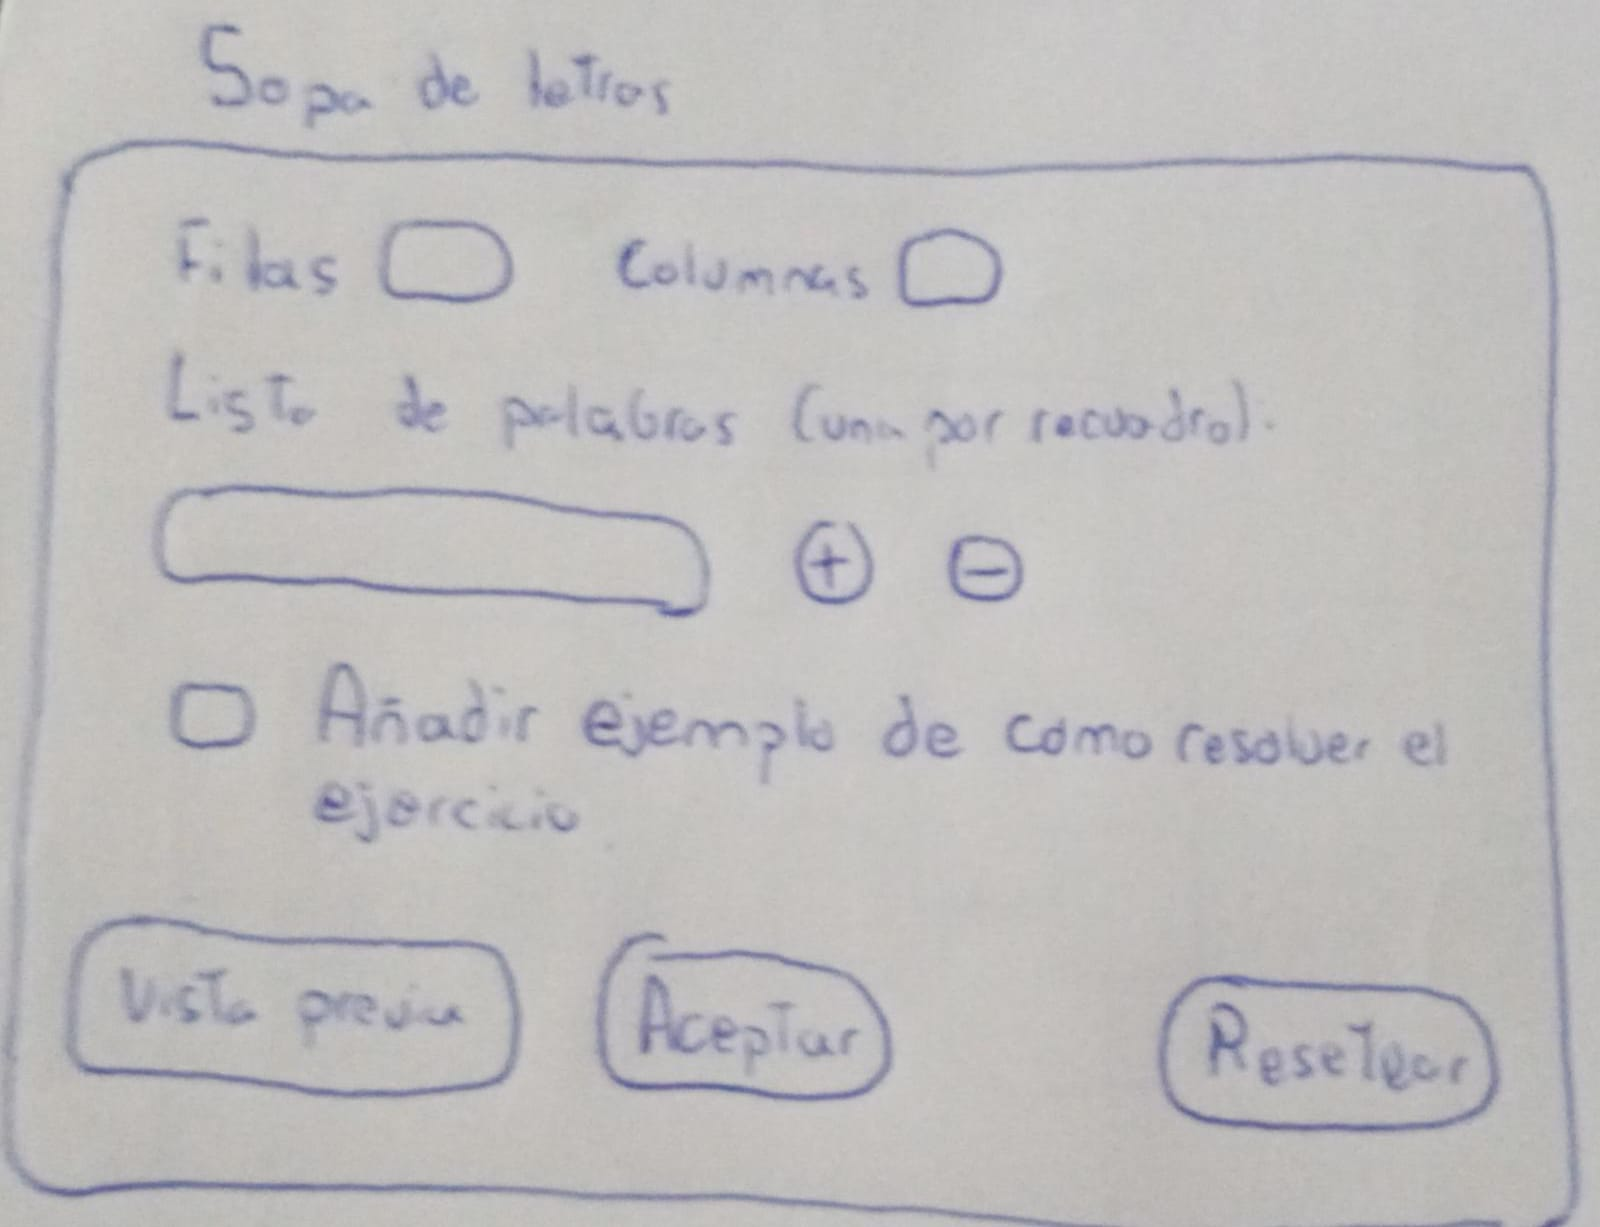
\includegraphics[width=0.6\textwidth]{Diseño/Johan/Johan6.jpeg}
    \caption{Diseño de página de sobre nosotros de Johan.}
    \label{Johan6}
  \end{subfigure}

  \begin{subfigure}{\textwidth}
    \centering
    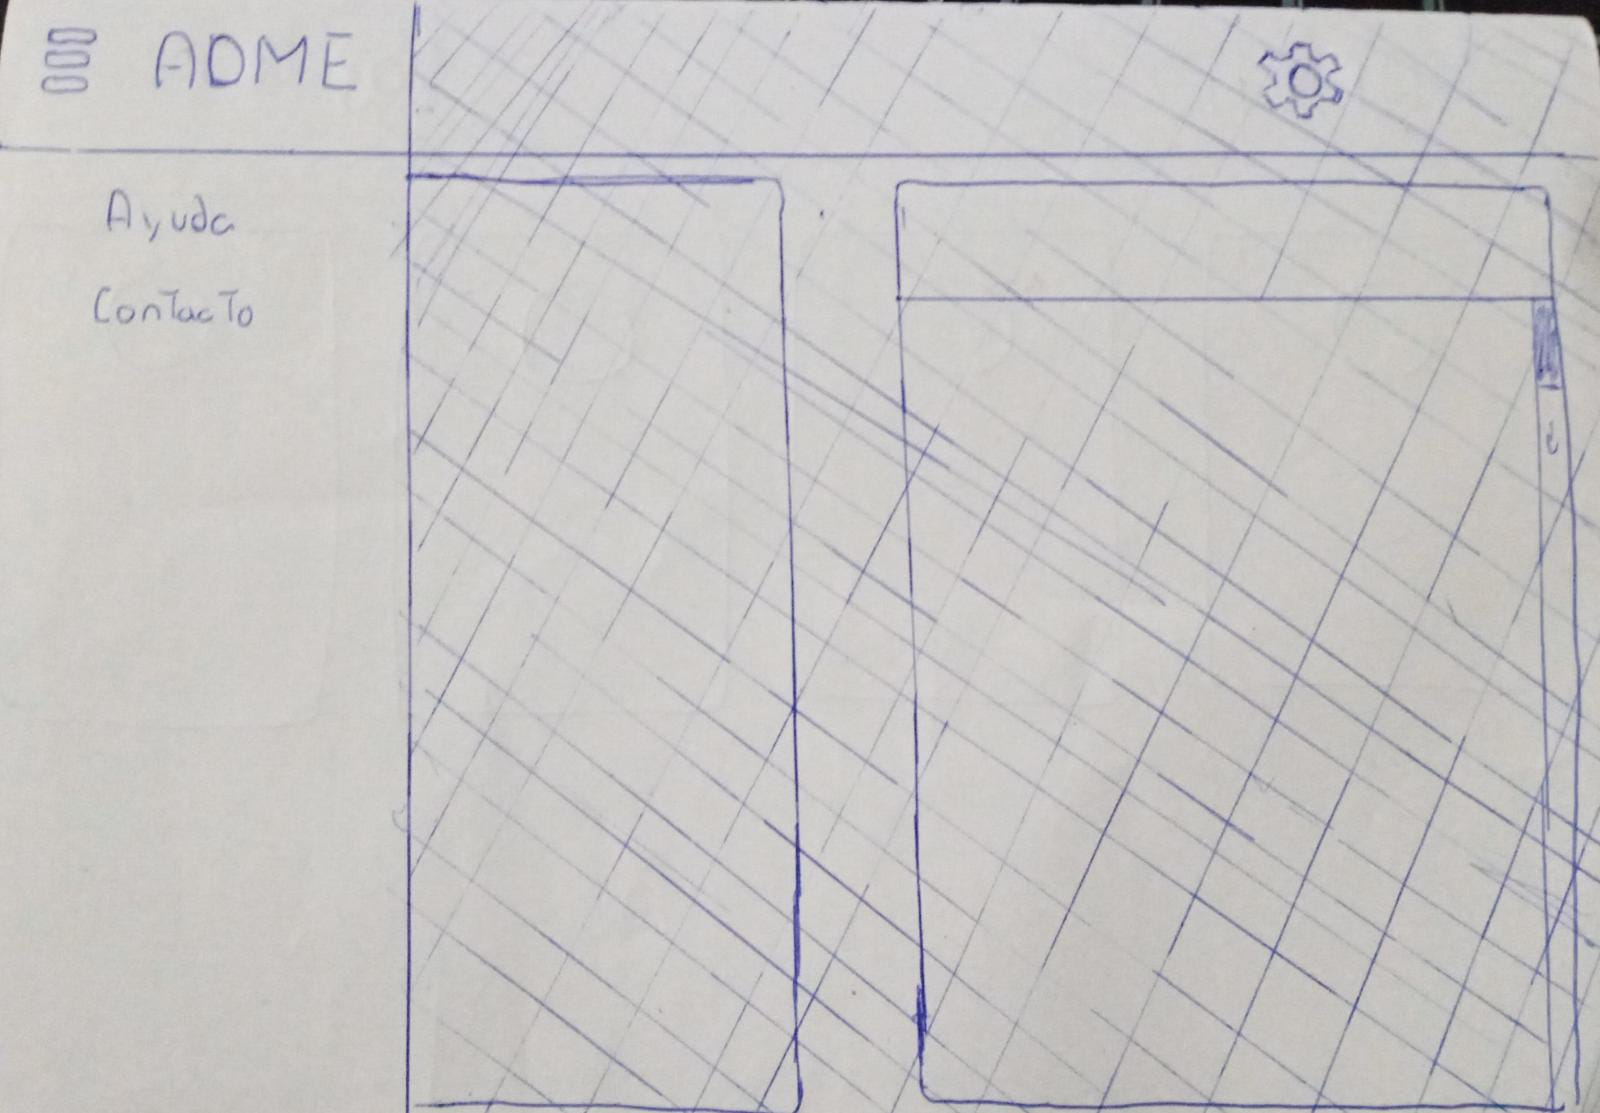
\includegraphics[width=0.6\textwidth]{Diseño/Johan/Johan7.jpeg}
    \caption{Diseño de barra de navegación de Johan.}
    \label{Johan7}
  \end{subfigure}

  \caption{Diseños de Johan Sebastian Salvatierra Gutierrez}
  \label{fig:disenyoJohan}
\end{figure}

\begin{figure}[ht!]
  \ContinuedFloat
  \begin{subfigure}{\textwidth}
    \centering
    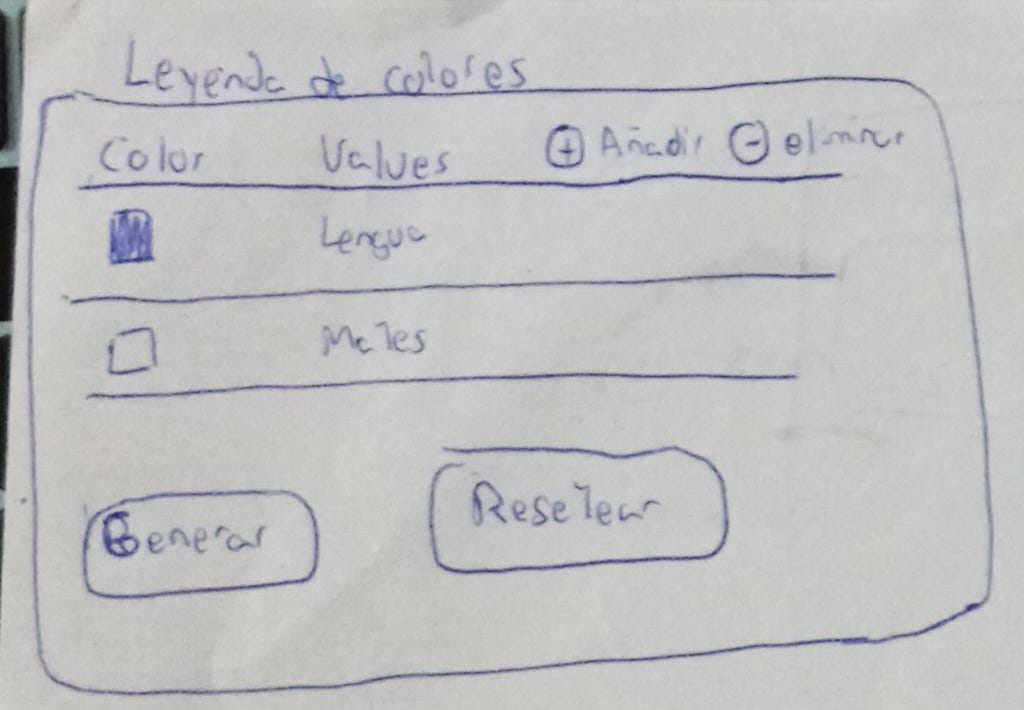
\includegraphics[width=0.6\textwidth]{Diseño/Johan/Johan9.jpeg}
    \caption{Diseño pantalla de inicio completa de Johan.}
    \label{Johan9}
  \end{subfigure}

  \begin{subfigure}{\textwidth}
    \centering
    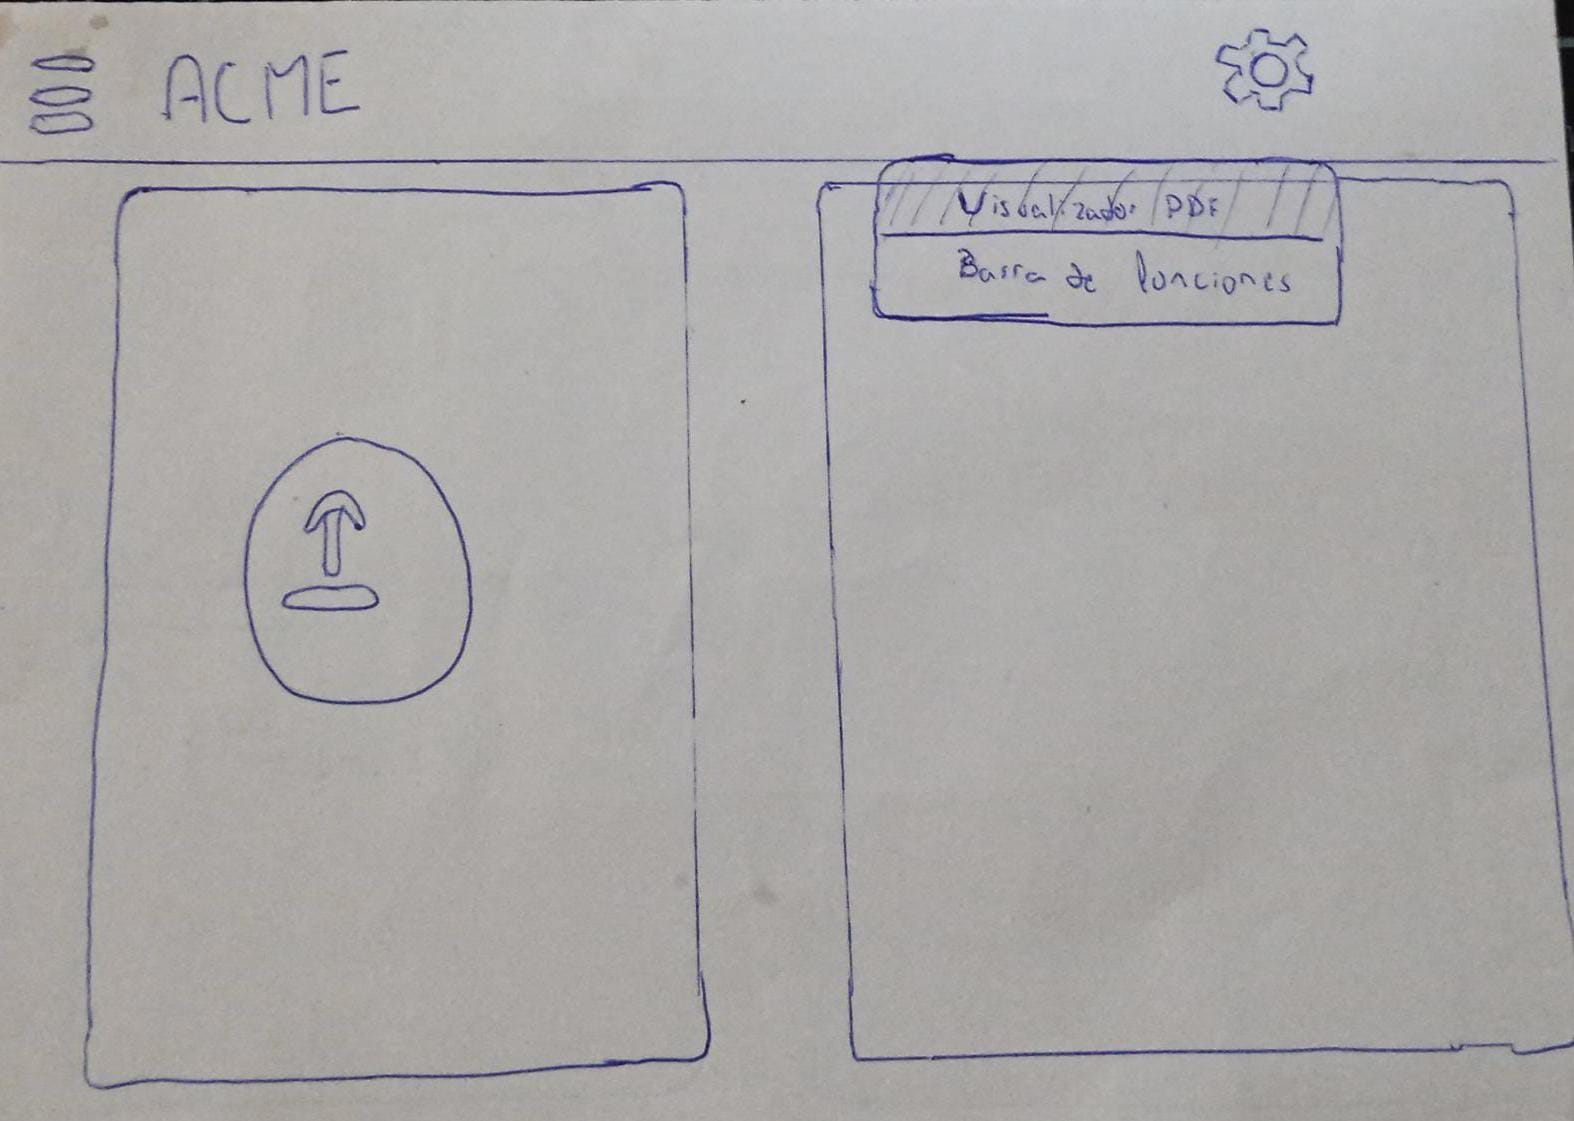
\includegraphics[width=0.6\textwidth]{Diseño/Johan/Johan10.jpeg}
    \caption{Diseño pantalla de inicio de Johan.}
    \label{Johan10}
  \end{subfigure}

  \begin{subfigure}{\textwidth}
    \centering
    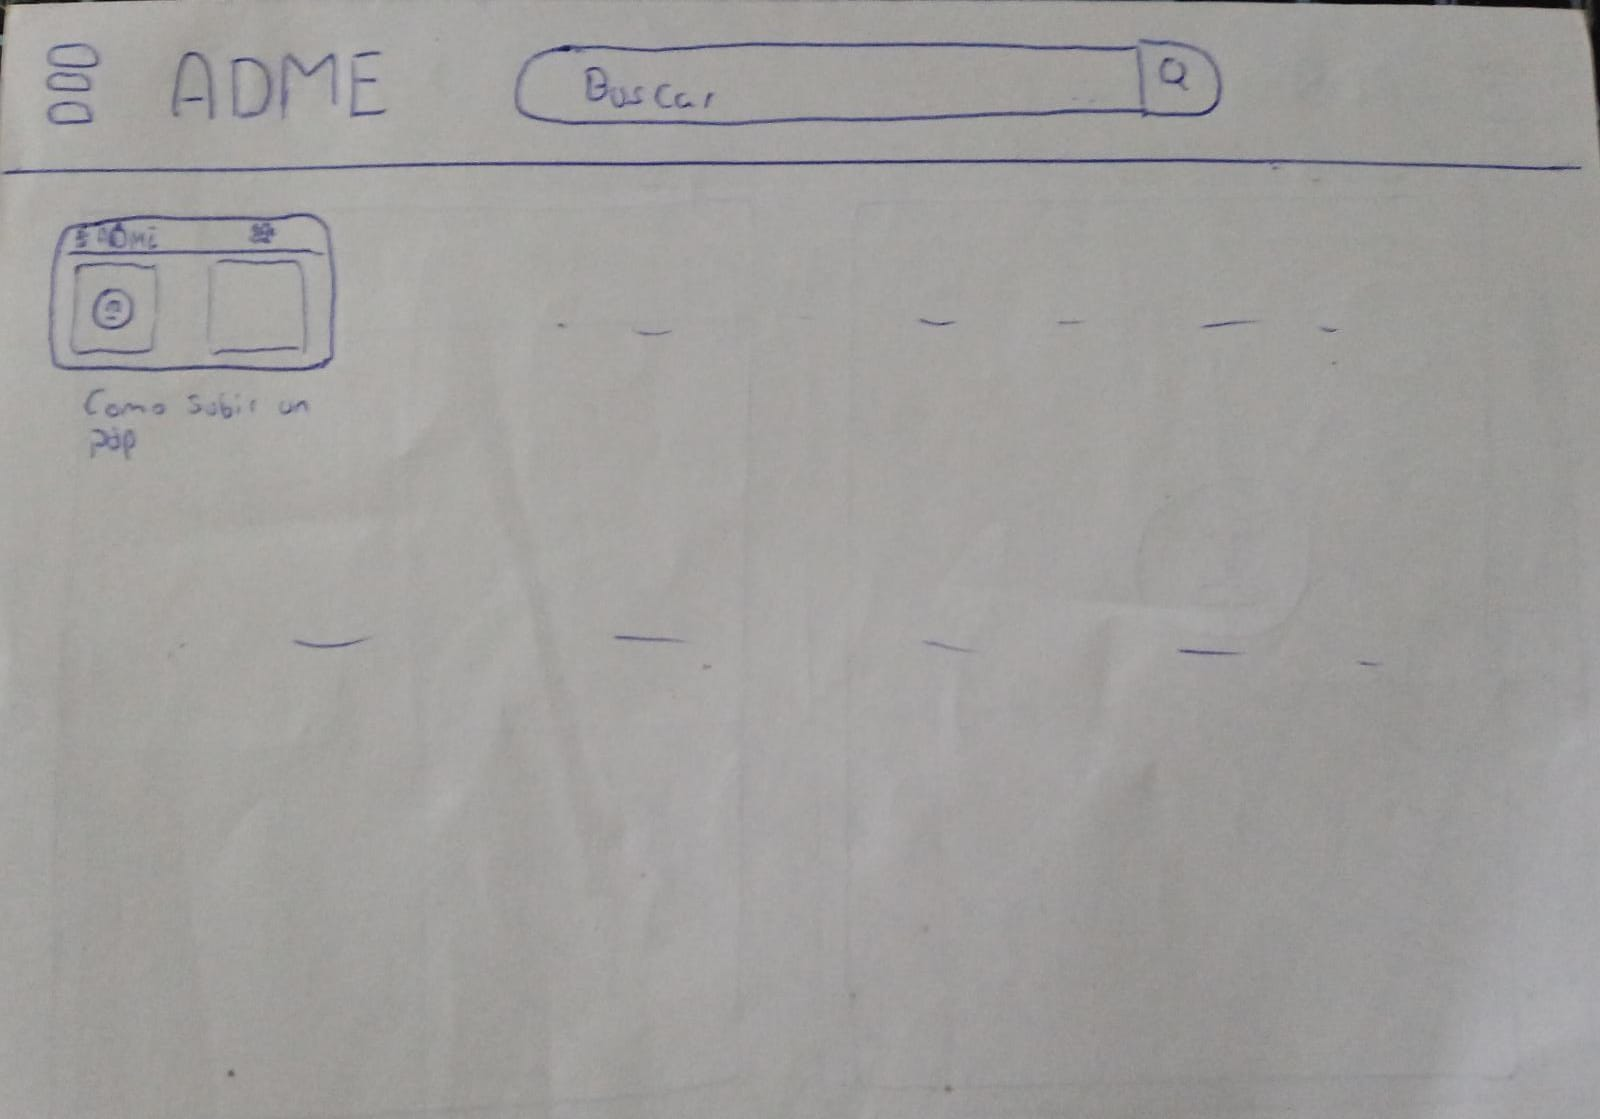
\includegraphics[width=0.6\textwidth]{Diseño/Johan/Johan11.jpeg}
    \caption{Diseño de página de información de Johan.}
    \label{Johan11}
  \end{subfigure}

  \caption{Diseños de Johan Sebastian Salvatierra Gutierrez}
  \label{fig:disenyoJohan}
\end{figure}